\documentclass[12pt]{report}

% includes
\usepackage{geometry}           % page size
\usepackage[utf8]{inputenc}     % encoding
\usepackage{palatino}           % font
\usepackage{graphicx}           % images
\usepackage{indentfirst}        % indentation
\usepackage[nottoc]{tocbibind}  % table of contents style
\usepackage[unicode]{hyperref}  % references from the table of contents
\usepackage{pifont}
\usepackage{amssymb}
\usepackage[dvipsnames]{xcolor}
\usepackage{comment}
\usepackage{tabularx}
\usepackage{multirow}
\usepackage[normalem]{ulem}
\useunder{\uline}{\ul}{}
\usepackage{enumitem,amssymb}
\usepackage{pdfpages}


%\usepackage[table,xcdraw]{xcolor} farge opå celler i table 
%\usepackage[showframe=true]{geometry}
%\usepackage{changepage}
%\usepackage[colorlinks]{hyperref}

% includes options
\geometry{  a4paper,            % scientific thesis standard
            left=3cm,
            right=2cm,
            top=2cm,
            bottom=2cm,
 }
\graphicspath{{images/}}        % path where the images are located
\setlength{\parindent}{1cm}     % paragraph indentation

% other options
\linespread{1.5}                % space between lines

% the document content
\begin{document}
    % macros (global)
    \newcommand{\uncheckedbox} {$\square$}
\newcommand{\checkedbox}{\rlap{\raisebox{0.3ex}{\hspace{0.4ex}\tiny \ding{52}}}$\square$}
    
    % front-matter
    \pagenumbering{gobble}
    
    % define the cover page
\begin{titlepage}
    \begin{center}
        % the university and faculty
        \large
        \MakeUppercase{KRISTIANIA UNIVERSITY COLLEGE}
        
        \LARGE
        \textbf{\MakeUppercase{DEPARTMENT OF TECHNOLOGY}}
        
        % the faculty logo
        \vspace{1cm}
        
\includegraphics[width=0.6\textwidth]{hk-logo}
        
        % thesis title
        \vspace{1cm}
        \Large
        \MakeUppercase{MASTER OF HUMAN-COMPUTER INTERACTION}
        
        \vspace{0.5cm}
        \LARGE
        \textbf{A Qualitative Assessment of Digital Nudging Intervention for Physical Activity}
        
        \vspace{0.5cm}
        \Large
        Synne Storhaug (706066)
        
        % Supervisor
        \vspace{3.5cm}
        \large
        Supervisor: Siri Fagernes 

        \vspace{1.5cm}        
        Restricted:
        \uncheckedbox Yes
        \checkedbox No
    \end{center}
\end{titlepage}
    \vspace*{\fill}

\vspace{1cm}
\begin{flushleft}

\large
\textbf{Acknowledgements}
% Your acknowledgement(s)    
%Who would you like to thank? 

%Thanks to my supervisor Siri. First and foremost for your passion for Human-Computer Interaction and your contribution to strengthen the awareness of this field in Norway. Also, for everything you taught me during this Master's degree, and for the guidance for this thesis.  

%Secondly I want to thank my dad, for playing an important role as supporter and adviser through my whole education. Couldn't have done it without you.

%I'd also like to thank my classmates, which I'm so proud of! Together, we are the first in Norway with this degree and are ready to conquer the future of technology.

%A special thanks to my one and only, Vilde, for holding up with me through thick and thin. Through the past two years, you have become one of my best friends, and I'm thrilled to share this professional interest with you.  

%In memory of my beloved grandmother, Karin Saus Larsen, who always believed in me, but never saw me complete the biggest thing so far in life. 

%Thanks to the rest of my family and friends for always supporting me and bringing positive energy.  

%Last but not least, a big thanks to the people of SATS, for making this research possible and believing in my ideas.  

\vspace{1cm}

% Certification of originality
I certify that the work presented in this thesis is my own unless referenced.


% Signatures and metadata
\vspace{0.5cm}

Date: ............................
\hspace{1cm} 
City: ............................ 

\vspace{0.5cm}
Signature: ....................................................................

\vspace{0.5cm}
Total number of words: .............................................

\end{flushleft}

\vspace*{\fill}
\pagebreak
    
    \chapter*{Abstract}

%Insert an abstract here.
Physical inactivity is one of the main factors for cardiovascular and non transmittable diseases in the world. In Norway, 70 percent does not follow the recommendations for governments (Helsedirektoratet). The utilization of technology and design, are important tools for reducing the numbers for physical inactivity. Personal Informatics (PI) and Persuasive Technology (PT) such as applications to monitor and motivate for physical activity becomes promising. Nudging is a term that has emerged from behavioral economics, and means ... As computer became commonplace, nudging was inherited to digital interfaces as well.  

 Digital nudge interventions have gained little attention when it comes to  user experience and perception, at least for physical activity promotion. Most studies regarding physical activity present measured efficiency through quantitative data and statistics (finne ut om dette gjelder bare for fysisk aktivitet eller DN generelt?)

Many nudging techniques have been identified, and there are therefore numerous ways to implement them. The question "how to nudge" remain unanswered. Many studies suggest that tailoring is a promising direction (hva grunnlag har de til å si at tailoring er så viktig hvis de ikke har gjort kvalitative stuider?? Finne kilder).

Describe context


\textbf{Keywords:} digital nudging, persuasive technology, informational health, gym app context, 
    
    % table of contents
    \tableofcontents
    
    \setcounter{page}{1}
    \pagenumbering{arabic}
    
    
    % chapters
    \chapter*{Motivation} 
%\section{}
%\subsection{}
%\subsubsection{}
%What was your motivation for conducting this study?

Two main / several factors amounted the motivation for this study. 

First of all, HCI role within health. 

Second, how physical activity recommendations are not persuasive enough,. 

    \chapter*{Abbreviations}

\begin{table}[h]
\begin{tabular}{|c|c|}
\hline
\textbf{Abbreviation} & \textbf{Description} \\ \hline
PT & Persuasive Technology \\ \hline
PA & Physical Activity \\ \hline
IS & Information Systems \\ \hline
TA & Thematic Analysis \\ \hline
GT & Grounded Theory \\ \hline
\end{tabular}
\end{table}

    \chapter{Introduction} 
%\section{}
%\subsection{}
%\subsubsection{}

%Introduce your topic.• State of the world…• The big BUT…• Therefore, we did…• The key findings are…• The contributions of this work are…

\section{Statement of Problems}

The state of the world is characterized by two major facts right now; 1) we are surrounded by (and dependent of) technology everywhere, and 2) physical inactivity is a global health problem. These two put together, serves as a fruitful area of interest for Human-Computer Interaction (HCI) researches. 

Many of our day-to-day choices are made on a digital interfaces, such as mobile application and websites. Smart phones, laptops, tablets and other technological devices are everywhere around us, and present us with choices, whether we are at work, school, home or on the go. The unlimited access to screens and other technological widgets has made mankind dependent on, and in many cases succumbed to, such devices \cite{mirsch_digital_2017}.
%(Digital Nudging: Altering User Behavior in Digital Environments)
This also implies that this type of user interface is powerful and can influence people in certain directions if designed carefully.  In fact, no system or technological interface will ever appear as neutral 
\cite{oinas-kukkonen_persuasive_2009}. 

In addition, recommendations from policymakers and other stakeholders are not sufficient in motivating people for more physical activity. On a global level the lack of physical activity is still a problem. Also, it seems that to fill in this gap is very difficult. Most experts argue that creating such changes is more important than ever. Inactivity have become a big killer in our society \cite{kohl_pandemic_2012}.

Most people are aware of the many benefits physical activity gives us, and the consequences of abstaining from this behavior. In Norway, we learn about why physical activity is good for us already in the childhood, and it continues through school, education and work. However, health statistics indicate that education is not good enough to ensure people to stay physical active on a regular basis. Numbers from FHI, show that only 30 percent of Norway's population fulfill the minimum recommendations of physical activity \cite{folkehelseinstituttet_fysisk_nodate}. %(Reference: https://www.fhi.no/nettpub/ncd/fysisk-aktivitet/voksne/) 
A questionnaire where participants where supposed to self-asses their physical activity level, revealed that about 30 percent of adults (20-85 years) in Norway are defined as inactive. However, comparable data have been measured with an accelerometer shows that 70 percent fall inside same category. These data are of higher quality than self-reported data (from experience one can gather that individuals have tendency to exaggerate opinions and behaviour that would put them in a better light). The large gap between self-reported and measured physical activity may imply that people are less active than they appear, or believe in (self-deception). (It should be mentioned that the number of participants for the self-reporting survey was low, which gives uncertainty about the data being representative of the entire population.) 

Norway is one of many countries which has committed to WHO's global goal of reducing inactivity. The concrete goal for 2025, it to reduce it by 10 percent \cite{noauthor_inaktivitet_nodate}.
%(Reference: https://www.fhi.no/nyheter/2018/ny-handlingsplan-skal-fa-folk-opp-av-sofaen/). 
The Norwegian Institute of Public Health (FHI), a Norwegian governmental agency subject to the Ministry of Health and Care Services (Helsedirektoratet), is in demand of an overview of best practices and initiatives that contribute to physical activity among Norway's population groups. These practices and initiatives could evolve from technology and user interfaces.

Although the recommendations regarding physical activity from the Helsedirektoratet is available in rich detail online, they still have the potential to become more accessible and embedded in everyday tools and services, such as technological devices. (However, it is not that simple.) Making education and information more available and persuasive will not alone drive the people at the wrong side of the scale into becoming enough physical active. The psychology of human behavior and absence of behavior is more complex than our ignorance. Visiting the field of behavior science, B.J Fogg insist that there are several factors that needs to be present at the same time in order to achieve a target behaviour; motivation, ability and prompt \cite{fogg_persuasive_2003}, is supposed to be the key to success. 

Take the scenario of a training center: all members are seemingly have the ability and some level of motivation to be physical active as they are already paying the monthly fee. Now, here is the challenge, how do we trigger or prompt them, into engaging in physical activity on level with the national recommendations? This is where technology comes in. It would be interesting to embed the knowledge from these stakeholders (FHI and Helsedirektoratet) into a digital context for people whoms motivation and ability is somewhat given. There are several ways to implement such an intervention. 
 
%This trigger factor is where we can utilize technology and user interfaces. Further Fogg describe three different variations of the trigger; facilitator, spark and signal. The latter is best to use when motivation and ability is present, (where considerations regarding tailoring, frequency and timing) \cite{fogg_persuasive_2003}.

%There is a need to make this information more available and persuasive. 
%Therefore it is interesting to embed the knowledge from these actors into everyday technology (for instance like an gym app). 

Persuasive technology is a well known concept in affecting health behaviours \cite{orji_persuasive_2018}.
Tracking, monitoring, sharing, social support, sharing, rewards and competitions are among the design principle to motivate physical activity through smartphones and wearables. However, such user interfaces may be perceived as intrusive and aggressive as they are based on theories of persuasion \cite{meske_status_2019}. 

Another design strategy that aims to influence behavior, is digital nudging . Its way of influencing behavior is slightly modest/careful way, by making people aware of the better choices and trigger reflective thinking\cite{meske_status_2019}.

So what kind of nudge should people be subject to, to change their behavior? This debate does not only revolve around making totally inactive people to become active, but ensuring those who are already active to continue on a regular basis. At the same time, we are aware of the 24 hour life, constant feed and the information overload. How do the technological and digital interventions survive in such environment? 

How do we reach the target audience with the message? What is needed for people to make use of a mobile application in general? The good user experiences. And in good user experiences there is often customized content. It has become an important design principle for making systems persuasive, and can therefore be transferred to digital nudging as well. Since digital nudging is quite new and in shortage  of qualitative research, we don't necessarily know how to tailor (it). In addition, digital nudging has not been implemented and studied in the fitness center context before. What applies to those users?

Among Norwegian citizens, 70 percent do not fulfill minimal recommendations of physical activity \cite{folkehelseinstituttet_fysisk_nodate}, meaning they are more prone to getting certain disease, illnesses and plagues, both physically and mentally, (than they need to be). The authorities and commercial players have a shared responsibility for ensuring good health among our population. Where to start? It seems logical to start a place where one is already on the right track (i.e. it is not about changing attitudes towards people as they are already motivated and aware of physical activity to a certain level). This study therefore approached the training center context, because here the users already have some of the prerequisites (motivation and ability) in order to achieve the targeted behaviour physical activity. Being member of a fitness center, does not necessarily mean that you meet the national requirements, at least not from week to week, because life happens, in short. This is therefore a suitable target group.

%For it to be sustainable, it should also be taken into account that the changes must be long lasting and preferably permanent.

This study will transfer theories from the field of psychology into digital nudging, in order to gain insight on users perception and experience of the given implementation, which again can contribute to establishing if this is an effective method nudging peoples choices about physical activity through digital environments. We are in particular investigating three aspects of the digital nudge intervention; 1) content , 2) message framing , 3) delivery method.  

%By performing a qualitative assessment of users perception of a implemented digital nudging intervention to promote physical activity. Aiming to gain insight and contribute with findings to the big overall question "how to nudge".

%There has been done several studies regarding the impact of communication, framing and other. For instance in context of persuasive systems, health communication system, behaviour change system, etc. It can remind and sometimes overlap the concept of digital nudging. However, to the best of my knowledge this is the first experiment including framing for digital nudging in specific. 

%Intro: verdens bilde: mer teknologi + mindre aktivitet
%Snu det om, bruke teknologi til å få folk mer aktive
%Tidligere forskning, persuasive design og tech etc... hva har blitt gjort ang fysisk aktivitet
%Vi har forstått at vi må ta mer fra pyskologien for å knekke design koden å kunne lage de beeste profuktene
%det er dette hci mye bunner i
%emrging trends: digital nudging, som faktisk stammer fra behavoirual ecomics..
%litt hva det er og som er funnet
%her er også spørsmålet: how to nudge?
%må låne ting fra andre fagfelt, gjøre tester av ulike mekansimer og ways of implementation, for å kartlegge for hvilke situasjoenr man bør benytte seg av hvilke type digital nudging. 

\section{Research Questions}
\begin{itemize}
\item RQ1: How are digital nudges based on consensus health information, experienced and perceived by gym members? 
\item RQ2: How does message framing affect the user perception of the digital nudge?
\item RQ3: How are push notifications experienced as the channel for broadcasting digital nudges? 
%\item RQ4: What should be taken into consideration for tailoring of digital nudges in this context? 
\end{itemize}

These questions are asked in order to answer the bigger problem statement: how to nudge and what to consider when tailoring digital nudges for physical activity promotion. The overall problem is thus how we should nudge, which implies that psychological effects should be exploited, how it should be implemented, how should content and framing be tailored, etc. The research questions is answered by qualitatively evaluating and investigating patterns, trends, tendencies, correlations. 
%interview data based on users perceptions,  
%Through this study I also aim at gaining insight into which factors should be considered when it comes to tailoring of digital nudges. 

\section{Aims}
The primary aim of the study is to understand user perceptions of the digital nudge intervention (taking message framing, push notification and content into consideration), in order to gather insight on how to tailor digital nudges and make them more effective in the given context. The gathered information will be used to strengthen and complement knowledge on nudging in general, and through digital environments such as mobile application. Such it will provide contributions to both academics, industry (commercial operators) and authorities. 

On the higher level, the aim would be to safeguard and improve public health by fostering good and healthy choices. This can be achieved by presenting and communicating health information and encourage the better choices through commonplace ubiquitous technology. This would be implemented using nudging mechanisms that build on psychological effects and processing. 

%multimodal interface  
%Making people life through new ways of applying HCI context, in set context health information, digital interface design
%Looking at how a certain implementation of digital nudging impacts attitudes towards regular physical activity by collecting qualitative data about users experience and perception

Further, the study aims to make HCI more prominent in the research field. Current research on digital nudging is mainly emerging from the view of Information Systems (IS) (e.g. e-commerce and organizational technology). This study approach the research area from an HCI perspective as it concerns the bigger question "how to nudge" by investigating the design of a implemented digital nudge interface and tries to understand users' perceptions and experiences. HCI's role is to investigate this to find out how this can become part of existing user interfaces or individual solutions to promote physical activity. This is mainly done in order to establish how to get closer to the answer to "how to nudge" and how to achieve effective digital nudges. The goal is hence to contribute to a better understanding of digital nudging from a HCI perspective in the given context and users, and identify the area that needs to be studied more closely. 

%To best of knowledge one of the first attempts 

\section{Objectives}
The objectives of the study were to design and perform a successful digital nudge implementation retrofit to an already existing technology (mobile application), and rolling it out towards a selection of users. Further, it was to conduct interviews and collect qualitative (and some quantitative) data about users perception and experience towards tested implementation, and evaluated from that perspective. More specifically what concerned the framing, the technology channel, content, information and source credibility. It was an ambition of the study to follow a normative and accepted standard and honor the integrity of the participants. 

\section{Research Design and Context}
\subsection{Context  }
%This study uses a qualitative research design (answering the whys and hows), where data are collected through interviews. 

The study was conducted in 2020, in affiliation with the Masters of Human-Computer Interaction programme in the Department of technology at Kristiania University College. This master thesis is conducted in collaboration with Sats, one of the biggest fitness centers in Norway, to investigate the defined problem statement in a context with gym members. Sats have gym centres all over Scandinavia, which makes them a useful partner which offers an opportunity to include a wider target population across country borders. However, considering the scope of this master thesis, the study was limited to only including Norwegian members due to physical attendance for interviews (which later was restricted to be digital based due to Covid-19). The study was carried out in the Oslo area in Norway.  

Through this study we are conducting a digital nudging intervention in a real-life context with gym members of Sats. The nudges will be sent as a push notification through the app that Sats distributes to their members. The push notification will only include text and no other visual effect. The Sats app main functionality is membership identification (QR scan to enter gym centers), booking group sessions and log training. However, it can be categorized as a persuasive mobile application as they are implementing different elements in order to increase motivation for physical activity, and to make their members become regular trainers. Such elements is for instance: challenges, social comparison, feedback, etc. 

\subsection{Target population }
%Aka: targeted users or population of interest.skal flyttes til intro? 
%Individer som oppfyller to av tre faktorer for å oppnå atferden, fysisk aktivitet. Ability and motivation. 

The target population for this study are individuals that have membership Sats. Based on the prerequisites about presence of ability and motivation, the target population includes almost (except people with injuries that stops them from engaging in physical activity or those who pay for the membership without any kind of motivation) everyone who is a member of a training center in Norway, which is a rather large group of people. It would be demanding to reach out for all of them, if not impossible. Therefore, there was made some frames and limitations in order to form a sample of the population. The sample population for this study consists of people with membership at Sats and that has downloaded their membership-app. The study sample is representative to its target population to some degree, as the participants varies in gender, age, motivation type, prior frequency of physical activity, attitudes, etc. (However, they do all belong to the same geographical area, as this was one of the frames for the sample).





    \chapter{Related Work}
%Testing av referanser \cite{acquisti_nudges_2017}, \cite{al_stairs_nodate} \cite{suri_stairs_2014}, \cite{fogg_persuasive_2003}, and \cite{hamper_behavior_2016}. +  \cite{karl_chapter_nodate}
%This master thesis had to adapt aims, objectives and research question after the pandemic hit Norway and caused problems with implementation of the study as it was originally designed. This chapter is strongly affected by this, and does therefore include some theory on topics (e.g. message framing) that are not elaborated on or discussed any further. 

This chapter aim to give an overview of supporting theory, relevant articles and topics that this study is founded on. As both persuasive technology and digital nudging are extensive research fields, the literature is limited to address mobile applications and physical activity promotion. This means that studies on nudging for wearables such as activity trackers have not been considered.

\section{HCI and Health}
Health is a prominent application domain and area of interest within the human-computer interaction field, both when it comes to health informatics, healthcare technologies and personal informatics for health and wellbeing 
\cite{wilson_human-computer_2015}
%(Reference: Technological Approaches to Promoting Physical Activity, HCI and mobile health interventions, HCI for health and wellbeing: Challenges and opportunities). 
There is a large potential for motivation, encouragement and the ability to change people’s health-related behavior through user interface design as people are becoming rapidly more dependent on technological and digital interfaces. Over the last decades, the development of health technology that promotes or helps people to physical activity has evolved from completely primitive step counters to wearable fitness trackers, often with a corresponding persuasive mobile application to visualize activity data (reference: ?). Now, the training apps evolves towards full integration with both activity tracker devices such as heart rate device, smart watches and gym membership. 

Evolution of technology for different health promotion started of with elementary step counters, large, clumsy artifacts that could be perceived as disruptive in everyday activities, to become step count as the most primitive functions that is embedded in almost all ubiquitous and wearable devices nowadays. Next were the more advanced fitness trackers, smart and pulse watches, and most recently development of persuasive mobile applications and versatile health wearables and integrated gym app.

Visualizing, tracking, monitoring and logging activity data motivates people to train more (reference). More recent design principles such as gamification, feedback, rewards, challenges/competitions and social influence has been embedded into the fitness devices
\cite{meske_potential_2019}.
%(Reference: The Potential Role of Digital Nudging in the Digital Transformation of the Healthcare Industry).
 
Around the peak in persuasive research (~2010), several articles aimed to give an overview of the technological approaches in different health related contexts. One particular article that mentions current and potential contributions in promoting physical activity at the time, was conducted by Maitland and Siek \cite{maitland_technological_2009}.
%(Reference: Technological Approaches to Promoting Physical Activity, 2009) 
Monitoring capabilities and activity inference techniques. Effective user experience. Applications that provide monitoring of physical activity often combine it with other different techniques to encourage users to be more physical active, for instance through goal setting, feedback and social influence. The article states that physical activity promotion and support systems have the power to lower the barriers for physical training, but cannot solve this challenge alone. Health education is another way of solving this problem, at least in certain parts of the world where demographic and technological prerequisites are fundamentally different.

\subsection{Barriers to Physical Activity} 
In order to understand how we can design effective nudges in digital contexts to promote physical activity, one need to visit the barriers which prevent or counteract physical activity. Such barriers are strongly dependent on several demographic parameters; age, gender, geographical location, nationality, cultural background, educational level, literacy, social and economic class and other\cite{sorensen_perceived_2008}.
%(Reference:Perceived barriers to physical activity across Norwegian adult age groups, gender and stages of change - ok å bruke den kilden? eller må man egentlig ha kilde på det?) 
Due to this, physical activity barriers are often researched within a limited scope, and with very specific user segments, such as diabetics, elderly, pregnant, college students, etc. However, it is reasonable to evaluate lack of motivation, information, time, resources, and injuries or disabilities, as “general” barriers for accomplishing physical activity independent of age and geographical location (Reference: physical barriers). Both lack of motivation and information (are examples where technology to motivate and educate is utilized) are manageable to overcome, because one can educate and/or motivate people through nudging. People suffering from serious diseases will probably not, to the same degree, benefit from nudging because motivation is hardly a factor. However, people that suffers from motoric diseases, chronic conditions or similar disorders that require self-management/care tools, could for sure be assisted by nudging \cite{rouyard_nudging_2018}.
%(Rouyard et al. 2018). 

\section{Persuasive Technology}
As mentioned in the introduction, a concept that is popular and accentuate nowadays, in all fields of informatics, design and psychology, is persuasive technology. Within this collective term there exists a numerous applications, systems and softwares, which intentions are to persuade users to act on something. That something could for instance be to stop smoking, drink more water or avoid snacking. Persuasive technology aims to change people’s behaviour, attitude or habits towards the most beneficial for the individual, through interactive systems \cite{orji_persuasive_2018}.
%(Reference: Orji and Moffatt 2018 - Persuasive technology for health and wellness: State-of-the-art and emerging trends)
Based on a variety of strategies and principles, the interface is designed to assist the user to gain motivation or interest for the sought behaviour change in a given context. This research field was introduced around 1990, by one of the discipline pioneers, B.J Fogg, a behavioral psychologist. His contribution became the very foundation for further research and proceedings. He stated that the power of designing for behavior change, should only be used towards enhancing society and people's life.

People are situated amongst and exposed to persuasive technology everywhere in the society, without necessarily being aware of it. The most typical application domains are education, traffic, sales, religion, sustainability, insurance, military and public health. The latter, persuasive technology influencing health and wellness, has received vast attention and lately expanded on its targets \cite{orji_persuasive_2018}.
%(Orji and Moffatt 2018) (Persuasive technology for health and wellness: State-of-the-art and emerging trends). 
For what pertains to health and wellness, two main directions have evolved; 1. disease management and 2. health promotion / prevention. Disease management hinges around enhanced self-monitoring and management for individuals that has already contracted an illness, injury or disease. It could for instance be self care technology for diabetics \cite{rouyard_nudging_2018}
%(Rouyard et al. 2018) 
or self medication to cure HIV \cite{schnall_mhealth_2015}.
%(Schnall et al. 2015). 
As for the other direction, i.e. persuasive technology for health promotion or prevention, it addressed the proactive and inhibitive aspects of physical and mental health. It could prevent diseases through promotion of physical activity or healthy dieting. It can also be used to encourage self diagnostics, e.g. self monitoring of mole cancer, breast cancer or similar, thus detecting symptoms at earliest  possible stage. In this thesis, I will mainly focus on health promotion and prevention, specifically physical activity promotion. 

It should be noted that the persuasive technology and design sphere in the health domain embraces several categories. There exist numerous different devices, ways of implementations, user interfaces designs, e.g. step counter, fitness trackers and other wearables, exergames, etc \cite{maitland_technological_2009}.
%(Reference: Technological Approaches to Promoting Physical Activity, 2009). 
However, this review will be limited to concern the physical activity domain and PT within mobile applications, as these are the more relevant to this master thesis. 

\subsection{Physical Activity Promotion}
According to authors X, motivation is a powerful factor when it comes to physical activity promotion. One study that underlies this \cite{hamper_behavior_2016}
%(Behavior Change Support for Physical Activity Promotion: A Theoretical View on Mobile Health and Fitness Applications) 
views mobile applications for behaviour change. From Fogg's behaviour model, we already know that motivation is one of the components that lead to behaviour. However, motivation is a complex matter as it could be a mix of both intrinsic (internal rewards; joy) and extrinsic (external rewards; appearance) factors. 

A quite recent review of persuasive technology for health purposes, identified 85 researches within 16 years of time 
\cite{orji_persuasive_2018}.
%(Reference: Persuasive technology for health and wellness: State-of-the-art and emerging trends, 2018). 
It stated that physical activity was the most researched health domain for persuasive technologies. However, only 15 percent followed an adequate qualitative research approach, which indicates that there are relatively few studies on user experience and perception when it comes to persuasive technology for health domain, including physical activity promotion. The effectiveness of different persuasive technologies was in particular investigated... 
Although different theories from behavioural science and motivational strategies were utilized, it appeared that persuasive messages, reminders and alerts (which all are relatable to digital nudge interfaces) were not identified in the research concerning physical activity. This further implies that a gap exist in the research.

Another study only reviewed persuasive technology for physical activity for mobile applications 
\cite{matthews_persuasive_2016}
%(Reference: Persuasive Technology in Mobile Applications Promoting Physical Activity: a Systematic Review, 2016). 
Articles regarding persuasive technology for physical activity was evaluated by using the PSD framework 
\cite{oinas-kukkonen_persuasive_2009}. Conclusion was that different design principles from the PSD framework seem to be dependent on each other. 

\subsection{Design Principles}
During the years of research on persuasion in technology (three last decades?) , different guidelines, principles and frameworks have developed. The study by Oinas-Kukkonen and Harjumaa\cite{oinas-kukkonen_persuasive_2009}
%(Reference: PSD: Key Issues, Process Model, and System Features), 
, is recognized and widely referred to in the field persuasive technology. It provided a framework for designing and evaluating persuasive systems. Four dimensions of support were identified; primary task, social support, dialog support and system credibility. Within these dimensions, 28 underlying design principles were announced. Some of these design principles will be reviewed. 

\subsubsection{Tailoring}
A prominent design principle within persuasion is tailoring, which have been widely investigated (Reference: Persuasive system design : State of the art and future directions). It belongs under the dialog support dimension, and refers to a systems ability to achieve higher level of persuasiveness when content and services are tailored to personal factors such as needs and characteristics, or contextual factors such as usage. Typically this data is information about country, language, location, etc. Using such data to personalize the service or application, are design principles that almost every commercial company take advantage of today. Online streaming services, webshops, grocery shops, travel agents etc all do it to different degrees. Commercial players are using these elements as effectively as they possibly can within the boundaries of technology and legislation. Thus health promotion initiatives involving nudging may have benefits of using same. No different from other applications. ln the health sector there is a fine line between what can perceived as commercial interest and libertarian paternalism. What is the motivation to implement it in any case? To get more engaged users, less hassle and time consuming, increase effectiveness. The effectiveness of the technology is the true measure of its value and relevance...

Other design principles from the PSD framework hinges around the dimension of system credibility. It is known that PT with features of system credibility will achieve higher level persuasiveness. Design principles belong to the Dialog support dimensions (such as reminders) could in fact remind of digital nudging.
 
 \subsubsection{Communication}
Whenever technology is used as a medium for persuasion, it becomes natural to visit the aspect of intentional communication \cite{torning_pdf_2009}.
%(Reference: Persuasive System Design: State of the Art and Future Directions). 
Fields of computer-mediated communication, rhetoric and psychology are strongly related to the HCI community, as they overlap and complement each other in the "how to design" questions. 

%Is the aim always to persuade? Is there different ways to persuade? Short-term and long-term? Is it about convincing the small and direct choices (here and now), such as whether you should go  training today or not. Or the long-term choices, to maintain a healthy and active lifestyle. 

Although one may say that research on persuasive technologies and communication had its heyday around 2009, it has remained an important topic and  branches into new directions. 

In fact, how we communicate is a powerful factor when it comes to technologies for behaviour change and nudging interventions (both offline and digital), since it often boils down to how the possible choices and directions are presented. One of the most mentioned communication strategies within this research area is framing, which will be elaborated  later on.

\section{Digital Nudging}
In recent years, a new strategy for design with intention has emerged in the siding of persuasive design; digital nudging. The concept refers to fostering people's behavior and choices through purposeful application of user-interface (UI) design elements in digital environments \cite{mirsch_making_2018}. Such elements could be graphics, wordings, contents, etc. and thus often represent simple and cost effective modifications in the user interface.

This design strategy origins from the term nudging within behavioural economics, and was coined in 2008 by Thaler and Sunstein\cite{thaler_nudge-_2009}. 
%(Reference: Nudge book). 
Back to the roots, nudging refers to influencing behaviours in desired ways through a deliberate presentation of choices, without using elements of coercion or changing economic incentives. In other words, preserving users freedom to choose is an important aspect of a nudge (i.e. easy to resist). Since then, nudging has frequently been applied for different purposes and domains, such as government (e.g. in the fight against the coronavirus) and health (e.g. hand hygiene at work). In the matter of fact, a clear/distinct/ application of nudging has been observed the past months, in the fight against the coronavirus. This proves the timely relevance of the concept. 

Gradually, different nudging techniques were passed on to technological and digital interfaces. Based on reviewed literature it seems that nudging through technological devices was first discussed around 2013 
\cite{thomas_nudging_2013}.
%(Reference: Nudging through technology). 
At this time, the concept was called technology-nudging, which embraced systems and technologies that aimed at helping users make better choices at individual and societal level (e.g. enhancing health), by providing necessary domain knowledge. However, it was not before 2016, that the term digital nudging was defined by Weinman, Schneider and Brocke \cite{weinmann_digital_2016}
%(reference: Digital Nudging, Weinman, Shcinerd, brocke)
now specified to the use of user interface design. Further, in 2017, digital nudging was introduced for HCI and IS domains
\cite{schneider_digital_2018}.
%(Reference: Digital nudging altering user behavior in digital environments). 
It is therefore a quite novel, yet prosperous, research area, touching upon several fields of expertise.

Several well-known concepts and cases can be considered as digital nudging (such as prompts, reminders, push notifications, etc). In fact, digital nudging often appears in practise, without consciously applying digital nudging strategies during design and implementation \cite{schneider_digital_2018}.
%(Reference: Digital nudging altering user behavior in digital environments, 2018). 
You may have noticed them without being aware, small subtle changes in the choice environment on your phone or at the web. Supposedly they are everywhere around us. 

As digital nudging is partly overlapping and share properties with principles/purposes of persuasive and behavioural design, it can be hard to distinguish between them (whether this is desired at all?). It appears that no successful attempt at delineating the terms by describing the real relationship between the two, has yet been made. The main difference between them seems to be that digital nudging is supposed to build upon psychological effects such as biases and heuristics\cite{mirsch_making_2018},
%(Reference: Making Digital Nudging Applicable: The Digital Nudge Design Method), 
(which is not the restrictions for persuasive design principles even though many of them does). It is also suggested that digital nudging actually performs a subspace of the design aspect if persuasive technology
\cite{schneider_digital_2018}. 
%(Reference: Digital Nudging: Guiding Online User Choices through Interface Design, 2018).
In addition, incorporated in the definition of digital nudging, is that the users freedom of choice must be honored. 

%One example of conventional nudging for physical activity promotion is; steps were painted at the staircase so that people would choose the stairs instead of the elevator (reference). 
%findings and insights from similar research fields such as behavioral economics and social psychology, and on similar concepts, such as persuasive technology, should be addressed.  

%Considering the novelty of digital nudging...

Despite the fact that digital nudging has been predicted as a fruitful research area for HCI\cite{mirsch_digital_2017},
%(Reference: Digital Nudging – Guiding Judgment and Decision-Making in Digital Choice Environments), 
the current literature (referring to digital nudging in its true state) is mainly limited to the IS field. The work by Caraban et al. appeared as a necessary step forward by highlighting different approaches for nudging through technology, i.e. contributing as a framework. However, it also states the need for more research in the direction of establishing a complete and common understanding of the design space. To the best of our knowledge there is a lack of studies that actually carry's out the design, implementation and evaluation  of digital nudging interventions (by its true forms), with the aim of understanding users' perception and experience of digital nudging.

%To the best of our knowledge, the research on digital nudging for physical activity promotion is also a thin literature for now. 

\subsection{Complexity}
Since the research of digital nudging is a relatively new art, the exploration of nudging is still developing. Whilst some aspects are covered, there are still things that we yearn to find, and the complexity of digital nudging emphasizes the need for extensive research. Some of the design aspects of digital nudging will now be reviewed...

\subsection{Digital environments and delivery methods}
Digital nudging unfolds within multiple digital environments; mobile applications, websites, wearables and other user interfaces\cite{mirsch_digital_2017}.
%(Reference: Digital Nudging – Guiding Judgment and Decision-Making in Digital Choice Environments). 
Hence, the concept of digital nudging is broad and includes several ways of implementation. This literature review will focus on digital nudging within mobile applications due to the scope of this research project. 

Even if digital nudging via mobile application may seem like a narrow variation of the art, it can still be implemented in different ways. It could appear from an internal source, i.e. integrated in the mobile app interface. Most often such nudges will aim to guide digital (in-app) choices, such as fostering users to make appropriate choices pertained to the app itself and/or the services it facilitates. One may regard this as an inherent quality of an app but it is predominantly related to digital choices. E.g. defaults options when setting up a new phone, opting users to make good choices w.r.t privacy and security, etc.

Digital nudges can also be delivered from an external source or database through different delivery methods (i.e. meaning it is delivered outside the app, as an additional feature). It can be described as content with the purpose of stimulating good choices that is associated with physical world and behaviours, e.g. push notification reminder to drink water (what we will refer to as external digital nudging). The content may consist of well known UI elements like text and graphics. 

When regarding the above mentioned categorization of internal and external digital nudging, it should be mentioned that those labels is not defined in previous literature, but it is our suggestion and contribution to the understanding of digital nudging, in order to distinguish the different variants that emanate from digital nudging. This thesis will focus on external digital nudging. 

\bigbreak
\bigbreak
\bigbreak

 As mentioned above, one of the aspect of digital nudging is the for which digital environment (also refereed to as technology channel \cite{mirsch_making_2018}.) it should be implemented in. 
 
%Another aspect of (external) digital nudges is the technology channel they are mediated through. Websites, mobile applications and wearables are examples of a technology channels \cite{mirsch_making_2018}. 
 
Further, nudging mechanisms could be implemented in different ways within the chosen technology channel. For example, in mobile applications the nudging mechanisms could be integrated into the user interface itself (e.g. defaults, online forms) or delivered to the user as external prompts (e.g. email, vibrations, SMS, in-app notifications, push notification, sound, light notification, digital badges, etc) \cite{purohit_functional_2019}.
%(Reference: Functional Digital Nudges: Identifying Optimal Timing for Effective Behavior Change). 
Purohit and Holzer \cite{purohit_functional_2019}
%(Reference: Functional Digital Nudges: Identifying Optimal Timing for Effective Behavior Change) 
discuss that more investigations are needed to establish which delivery method should be utilized for specific target behaviors. In order to design effective digital nudges, an assessment of available technology channels and delivery methods should be conducted\cite{mirsch_making_2018}
%(Reference: Making Digital Nudging Applicable: The Digital Nudge Design Method). 
It is important that the chosen technology channel and delivery method are familiar to its audience. It might be the case that different methods are experienced differently in terms of credibility, intrusiveness and usefulness to users. %Looking at other qualitative studies on the user's experience of the various technology channels and delivery methods could be useful. 

%For physical activity promotion, the use of text messages is widely researched (however not as nudging) (reference: Efficacy of text messaging-based interventions for health promotion: A meta-analysis). 

To the best of our knowledge, there are no studies scrutinizing push notification as delivery method for digital nudges even though several studies mentions it as a commonly used\cite{dhar_persuasive_2017}. This may be due to the novelty of research, and because many of the examples of nudging observed in practise are in fact are unintentional \cite{mirsch_digital_2017}. 

%(Other considerations is as mentioned timing and frequency, however, this was not the focus for this thesis.) 


However, relevant studies state that the use of push notifications should be carefully considered, to avoid being perceived as disturbing or troublesome to users \cite{warren_push_2014}
%(Reference: Push Notification Mechanisms for Pervasive Smartphone Applications). 
The article mentions how the use of push notifications has increased in marketing, to push advertising and offers to users. Other typical use of push notifications is to remind the user to interact with the (sender) app, i.e. to increase user engagement, which is a challenge regarding health promoting apps \cite{bidargaddi_prompt_2018}
%(Reference: To Prompt or Not to Prompt? A Microrandomized Trial of Time-Varying Push Notifications to Increase Proximal Engagement With a Mobile Health App).

\subsection{The many facets of digital nudging}
Some researches have aimed at identifying different types of nudges, and for which situations they are most effective. However, it seems that there is a lack of consensus when it comes to the different types of nudging, due to researchers from different communities defining new and different types in a rolling manner. Furthermore, the labeling of the nudge categories does not match even though they talk about the same concepts. 

Sometimes nudging can be difficult to identify as it overlaps with other design strategies and principles. To make it even more complicated, nudging is more like an umbrella term that comes whit a number of different appearances and facets. Through the systematic review on technology mediated and digital nudging by Caraban et al.\cite{caraban_23_2019}, 23 distinct mechanisms were identified. The mechanisms where classified in six different categories: facilitate, confront, deceive, social influence, fear, reinforce. 

\begin{itemize}
\item Facilitate: nudging mechanism, reduces people's physical or cognitive effort, hence facilitating for decision making. It is based on the status-quo bias which refers to that humans tend to go with the option with least resistance.
\item Confront: nudges introduce doubt when people are about to make a decision. It exploits the regret aversion bias, which means that people are extra careful in a situations where risk is perceived. By breaking mindless behavior and make suggest using the reflective mind. 
\item Deceive: nudging mechanism adds inferior choices so that a particular choice is promoted harder than the others. 
\item Social influence:  nudge takes advantage of what people believe is expected from them, such as adapt to or accept certain norms or social rules. 
\item Fear: Nudges in the fear category, uses the feeling of fear or loss to make... 
\item Reinforce: repeat actions to learn reflective thinking. 
\end{itemize}

Further, Caraban et. al \cite{caraban_23_2019} makes an attempt to define in which situations the different nudging mechanisms should be used. Through Fogg's behavior model they are able to categorize all the 23 nudging mechanisms in one of the three forms: facilitator, signals and sparks.

\begin{itemize}
\item Facilitator (ability strategies): makes an task or a choice easier for users. Reducing distance and effort. 
\item Spark (motivational strategies): says to be optimal in situations where the user lack motivation 
\item Signal (trigger strategies): optimal in situations where the is a divergence between a users intention and actions, but where motivation and ability is often present. 
\end{itemize}

Despite the research already covered on the topic, a complete overview of the different types and implementations of digital nudging is still missing. Other researchers have categorized nudging in a different approach, sorting them within other types of labels. For example, Jespersen and Hansen\cite{hansen_nudge_2013}, defined four different classes where they categorised the nudges in. %(Reference: Nudge and the Manipulation of Choice. A Framework for the Responsible Use of Nudge Approach to Behaviour Change in Public Policy). 
Two questions determines their four classes: if the nudge is aimed at the reflective or the automatic mind, and if the nudge is visible for the user or not (also called transparency). This creates four intentions of nudges; influencing behavior (automatic-transparent), prompting reflective choices (reflective-transparent), manipulate behaviour (automatic-non-transparent) and manipulate choice (reflective-non-transparent) \cite{hansen_nudge_2013}.

Since different categories and labels are used on seemingly similar nudging mechanisms, it seems that there is a need of a structured overview of the digital nudging hierarchy. 

\textbf{Signals }
In order for nudges, belonging to the category of signals, to result in the achieved targeted  behavior or decision, some variables should especially be considered. Those variables are timing, frequency and tailoring \cite{caraban_23_2019}. A signal should appear in the right moment in order to be successful, however, what characterizes the right moment will depend on the situation and purpose of the nudge. Caraban et al. also claims that frequency may affect the effectiveness of the signal. In addition, another study showed that tailored signals / prompts / reminders / nudges with higher frequency are more effective than generic prompts with rarer frequency \cite{fry_periodic_2009}. 
%(Reference: Periodic Prompts and Reminders in Health Promotion and Health Behavior Interventions: Systematic Review). 

%Within tailoring, it also appears different variables (for instance content and framing), which leads us on to the common design principle of persuasive design. Which we are describing later on.  
Could be similar to prompts, push notifications, reminders, etc, as can be seen as features within persuasive technology. 

\subsection{How to nudge?}
For design of user interfaces in general there has been developed numerous of guidelines, principles and frameworks. Putting nudging elements into the user interface design must be done thoroughly. The user interface design will always have the ability to steer people in certain directions\cite{schneider_digital_2018}. 
%(Schneider, Weinmann and vom Brocke 2018 Digital Nudging:Guiding Online User Choices through Interface Design). 
What we choose is dependent on how the choices is presented. Due to limited cognitive ability, not always acting on rational behaviour, biases affect our decision making. Designers of behavior change systems (or other similar systems) has the ability to present the choice environment in a certain way to gently push users into a certain direction. 

What holds for step 3; design the nudge, is of deeper interest. Schneider further advise the designer to choose the suitable nudging mechanism in order to steer the users towards the defined goal and targeted decision. Even though the article mentions different tools and frameworks one can make use of for choosing mechanism. 

One of the first attempts at providing a framework for nudging in offline settings was the work by Ly et. al 
%(A Practitioner’s Guide to Nudging) 
in 2013 \cite{ly_practitioners_2013}. It aims at making the process of implementing nudging more accessible, by suggesting a four step model; 1. map the context, 2. select the nudge, 3. identify the levers of nudging, 4. experiment and iterate. As we know, when computing became commonplace nudging was inherited to the development of information systems as well. In 2017, Meske and Potthof introduced the DINU model \cite{meske_dinu-model_2017},
%(reference: THE DINU-model—A process model for the design of nudges),
a process model for implementing nudging in the field of IS, which are strongly related to HCI. It propose a three phase process for designing digital nudges based on knowledge from the research area of nudging, but also from persuasive technology and theories of persuasion; analysing, designing and evaluating. 

Further, Schneider, Weinmann and vom Brocke \cite{schneider_digital_2018}, made suggestions on how to utilize the digital context of web sites and apps for implementing and designing nudges .
%(Reference: Digital Nudging: Guiding Online User Choices through Interface Design, 2018). 
Their idea was that much of what applies to nudge designs in offline contexts can be inherited into digital contexts, as all choices are affected by human heuristics and biases. Furthermore, they emphasize that digital contexts not only consist of online consumer choices (an example they use a lot), but also systems, applications and websites related to e.g. health and social media. The proposal could therefore remind of the process that is followed when developing traditional information systems and other applications; 1. define  the  goal, 2. understand  the  users, 3. design  the  nudge,  4. test  the  nudge. 

Using the work of Meske and Potthoff 
\cite{meske_dinu-model_2017}
%(2017) 
and Schneider et al. 
%(2018) 
\cite{schneider_digital_2018}
as inspiration, Mirsch et al.\cite{mirsch_making_2018} developed a new method for digital nudge design, that was empirically validated and targeted for practitioners such as UX designers and similar.
%(Reference: Making Digital Nudging Applicable: The Digital Nudge Design Method). 
They claim that the reason why implementation of digital nudging is nearly absent in practice, is due to lack of awareness and a systematic design approach for it.

More recently, Caraban et. al \cite{caraban_23_2019} enlighted the “how to nudge”-challenge from a more HCI perspective, by reviewing the current design space of nudging mediated through different technological prototypes. Through their work they concluded that even though existing frameworks 
%(References: Beyond Nudge, Digital Nudging 2016 - Schneider, The Mindspace Way, Hansen and Jespersen 2013) 
brings valuable insights about cognitive biases and nudging mechanisms, they are not providing a complete answer for the “how to nudge” question. Nevertheless, Caraban et al.’s own work contributes in connecting these two aspects, about which cognitive biases and which mechanism should be used to achieve the desired behaviour or choice. Their identification of nudging mechanisms serve as a framework for researchers and practitioners when developing and designing technology-mediated nudges. 

\section{The Psychology behind }
What makes persuasive technology so powerful? One of the answers in order to manage and understand this, is the fact that it builds upon theories from both psychology, cognitive science and behavioral economics. Together with developed design features and principles within persuasive design, it underlie how the technology is experienced and perceived as convincing. Firstly, I will describe some of the essential details from psychology that aims to explain how people think, and then some design principles and motivational strategies, in the following paragraphs. 

\subsection{The Dual Process Theory}
Human decision making is compounded process. The Dual Process theories of decision-making is an important contribution in order to understand the human behavior \cite{caraban_23_2019}.
%(Caraban et al. 2019)(reference:  Thinking Fast and Slow). 
Humans have two modes of thinking: the automatic and the reflective. The reflective system is based on rational processes and shaped by consciousness. This means that it is slow, effortful and goal-oriented. According to Craban et al. \cite{caraban_23_2019}, most of HCI research (94 percent) on nudging through technological and digital interfaces focuses on this way of thinking when exploiting the effects of nudging. Nevertheless, it is the automatic system which is used in most cases during a day (95 percent). It is responsible for repeated and skilled actions, and works therefore quick, needs minimal effort, and is based on instinctive. Including research on the automatic system in the context of nudging, is referred to as an untapped areas of opportunity.

Humans are irrational and tend to take choices accordingly. Sometimes we need a gently push in a certain direction, to take more sustainable, healthy and expedient choices for ourselves and the society. Inactivity and public health is a worldwide problem  and  is  often  used  as  the  purpose  to  study  the  effects  of  nudges.  Most  studies regarding physical activity promotion exploits the reflective mind, whilst the idea of being able to promote motivation for physical activity to be handled by the automatic system could be revolutionary. In fact, the literature rise questions if technologies can rely less on users will and capacity to engage, meaning exploiting the automatic system.  

\subsection{The framing effect}
Human forecast is proven many times to be biased, and our decisions is inveigled by cognitive biases and flawlessness  \cite{thaler_nudge-_2009}.
%(Reference: Nudge Book). 
Nudging can help the individual to make optimal choices by detaching from systematic cognitive biases.
%(Reference: Nudge Book). 
Our decision-making is therefore influenced by how the choice is presented, i.e. its framing. Framing could for example be the use of different situations, wordings or consequences, to convey a message so that it is presented in a way that makes the choice more attractive for the user. 

One way of utilizing the framing effect is through message framing/wording of a message. Message framing, meaning how the message is presented, either with the positive consequences (gains) of a certain action or the negative consequences (losses) with the absent of that action \cite{rothman_shaping_1997}.
%(Rothman and Salovey, 1997). 
To understand the effect of framing fully, it is necessary to visit other theories within psychology that strongly relates to framing. Prospect theory makes statements about gain-frames and loss-frames as to which is better to use faced with a quantity of risk, e.g. often denoted as small risk or large risk (smaller or bigger evil)
%\cite{kahneman_prospect_2012}.
%(Kahneman and Tversky, 1979). 
In context of physical activity promotion it can be translated to the large risk being the risk of contracting a health condition with the ultimate consequence of (early) death. The small risk can be interpreted as the time wasted in the gym should this information not be correct. Under such circumstances theory states that individuals a willing to accept the small risk (e.g. waste time in training) to avoid the big risk (early death) and that positive framing is favourable. 
%This is also reflected through loss aversion bias, which claims that there are stronger reactions and emotions associated with a loss than a gain (reference) .

In the context of health related behaviours, message framing has in particular showed to be effective. For example, nudging people to do self examinations for skin and breast cancer (detection behaviour) have proven to be best when the framing of the message enlights the increased risk in the absence of it, and not the reduced risk if they actually do it, i.e. loss-framed \cite{thaler_nudge-_2009}.
%(Reference: Nudge book). 
On the other side, several studies conclude that in contexts of preventative health behaviors (such as skin cancer screening, smoke cessation, physical activity), gain-framed messages are measured to be most effective compared to loss-framed \cite{gallagher_health_2012}.
%(Reference: Health Message Framing Effects on Attitudes, Intentions, and Behavior: A Meta-analytic Review)

A systematic literature review on existing nudging research (primarily offline context) reveals that framing is widely researched within promoting health related behaviours
\cite{mirsch_digital_2017}
%(Reference: Digital Nudging: Altering user behavior in digital environments). 
However, the article states that little is known about framing and other psychological effect in digital nudging contexts, and questions whether the effects from “conventional” nudging are transferable. 

Message framing has been explored for several purposes, but it seems it has been most researched in the context of health messages related to persuasive systems and behavior change systems. There is a lack of research regarding digital nudging and message framing... However, since we are investigating digital nudging often comes in the form of a text message or notification, it is important to include the mentioned research when scrutinizing digital nudging as well. 

Rezai et al.
%\cite{rezai_developing_2017}
%(Developing Persuasive Health Messages for a Behavior-Change Support-System That Promotes Physical Activity) 
investigates the topic of tailored persuasive messages that pertains to ergonomics. This research is still an ongoing project, where the referred article is the first of three parts. The experiment aims to examine the effects of tailored messages from a behaviour change support system that promotes physical activity. The user segment comprise participants in the age 18-30y, who have a sedentary lifestyle. The experiment entails three different types of messages, one focusing on the positive aspects of exercising (gain), and two on the negative aspects of not exercising (loss) with a difference in??. To develop and define a set of validated health messages was the goal of this particular study. Findings were that messages focusing on the benefits of being physically active (gain-framed) was the most persuasive for this user segment. The first loss-framed message that highlighted what a person could avoid by being physically active, was perceived as the second most persuasive. The second loss-framed message, pinpointed the consequences of not being regularly active, which had the least impact. The study was conducted as an online survey, and that the persuasive health messages were presented on a digital surface as such. The messages were not tested in a real life scenario, merely by feedback, i.e. it was not checked if the users actually responded in a physical manner (however this is hard to measure). The fact that this article was published in 2017, and that the findings offspring further studies, underpins the relevance of it. Though this study focuses on persuasive messages, and not nudging in particular, it is still relatable.

A recent article from 2019 
\cite{williams_effects_2019}
%(Reference: The effects of message framing characteristics on physical activity education: A systematic review) 
provided a systematic review on message framing in regards of physical activity. Effectiveness of messages was investigate for 13 studies with overall healthy adults as participants (one study with overweight) were included, based on quantitative data and statistics. All of the reviewed studies did test gain vs loss + one other message framing characteristic which varied, focusing on increasing the participation of physical activity. The findings conclude that gain-framed messages is most effective in the context of promoting physical activity, which is consistent with previous research. They mention that more research should be done on gain vs loss, including other message framing characteristics to strengthen the evidence of message framing and to expand the participants.
%This indicates the lack of qualitative research on the topic. Mention…  
The importance of this review lies in the fact that health professionals trying to influence physical activity behavior change should be able to use message framing to increase their effectiveness.

\subsection{How to measure the effect of nudging?}
Researchers and practitioners are asking how we should design effective nudges 
\cite{purohit_functional_2019},
%(reference: Functional Digital Nudges: Identifying Optimal Timing for Effective Behavior Change),
but what is meant by effective nudges, and how do we measure them? Effectiveness refers to the degree to which the given intervention has persuasive ability, and there is a distinction between actual and perceived effectiveness 
\cite{dillard_relationship_2007}.
%(reference:, The Relationship Between the Perceived and Actual Effectiveness of Persuasive Messages: A Meta-Analysis With Implications for Formative Campaign Research). 
When we talk about perceived effectiveness, this is the user's own perception of the effect, i.e. the probability of the nudge to have a persuasive impact. Whereas actual effectiveness is the measure of the true impact the behavior or choice, which is done by applying quantitative research methods, collecting statistical data. The reason that many studies use or refer to perceived effectiveness is because it is difficult or almost impossible to measure actual effectiveness since behaviour is prone to several influencing factors. It is especially difficult to measure for digital nudging interventions aimed at physical activity promotion as would require activity meters. Besides, a quantitative research approach does not provide the full picture and understanding on why it worked or not. 

%hvor skal denne? when nudging fails
However, when regarding digital nudging, it should might not be measured in the same way as other behavior change technologies. Caraban et al. also discuss main factors to why nudging fails. One of them is the perception of intrusiveness. People may feel their autonomy is taken away. Nudging that only mobilize the automatic processing can cause users to learn nothing from it (since they haven't reflected on the choices). That is, in situations where the users are not exposed to the nudge, they will not be able to make that choice independently (because it was taken automatically through the influence of the nudge). 

\section{(Ethical) Implications and challenges}
The benefits one can gain from digital nudging and persuasive technology are apparently many and has gotten much attention. However, there are several ethical considerations to be aware of when implementing digital nudging. The lack of ethical considerations within research on persuasive technology is addressed by Torning and Oinas-Kukkonen 
\cite{torning_pdf_2009}.
%(Reference: Persuasive system design : State of the art and future directions). 
In addition, studies scrutinizing nudging often mention these concerns, however they are claimed to only be grasping the surface of the problem. 

The definition of a nudge as Thaler and Sunstein defined it back in 2008, claims that it shall only be used for good incentives, i.e. for the users best interest \cite{thaler_nudge-_2009}. It is useful to question whether this is always the case. As with any other emerging technology, it may be exploited beyond its intentions. And even for the concern of increasing physical activity, is that really the best behaviour for every individual user? That discussion belongs to another discipline (philosophy) and we will leave it with that. 

\subsection{The fine line between persuasion and manipulation}
Through the review on digital nudging literature, both academic and business related, ambiguity is perceived about what constitutes as nudging and what is pure marketing. One of the nudge criteria is to safeguard the user's freedom to choose. It seems that the term nudging is often used incorrectly in business related contexts. 

By revisiting the categorization of nudges through Jespersen and Hansen framework 
\cite{hansen_nudge_2013}, we see that nudges under the “automatic-non-transparent” category is said to manipulate behaviour. Such mechanism of nudging (e.g. subliminal priming, opt-out policies, adding inferior alternative, deceptive visualization, biasing the memory \cite{caraban_23_2019}) is often unrecognized, and may therefore deceive users. This rise questions whether or not that category could actually embrace nudges, as users freedom to choose is not safeguarded. Examples of this is when nudging is used in commercial purposes, when the user is influenced to use money, take a choice that is not for the users best interest, but rather for the organization or company behind. Such nudge implementations are unfavorable and void way of implementing a nudge, due to its ethical implications. Transparency is important to avoid manipulation \cite{karlsen_recommendations_2019}. 

\subsection{Criticism }
Many studies praise the effect of nudging, and sometimes it seems that nudging is always a good idea. Some researchers \cite{matjasko_applying_2016}
%(reference: Applying Behavioral Economics to Public Health Policy: Illustrative Examples and Promising Directions) (Matjasko et al. 2016) 
are more critical and questions the effects of nudging and discuss drawbacks and limitations. The first point of view is that the term nudging is vague and thin. (It should be noted that the article was published in 2016, and much has happened since then.) However, it also mentions that some interventions that goes under the category of nudging in fact should be described otherwise. Further, the authors speculate that nudges may lose effectiveness over time. It refers to studies where nudging in fact seems to have small and short lived effects. These findings contradicts what many other researchers believe, that nudges have a great potential. Research on the long-term effects of nudging is minimal and lacking to contradict these findings. Lastly, this article mentions that in order to become more successful, tailoring of nudging is needed. 

\section{Summary}
Through this literature review, it emerges that digital nudging is a broad concept with many underlying directions. It has also made us aware of the many needs and shortcomings in the research area. Firstly, a concise overview describing the various concepts (digital nudging, persuasive technology, behavior change systems and similar) and the connection between them should be developed to get a common understanding of the terms and how they relate.

Furthermore, it appears that the design aspect of digital nudges is extremely complex, thus a map describing the different paths within digital nudging is needed, in order to better understand which mechanisms and delivery methods (and other design aspects) that should be utilized in which situations. There are made some contributions i form of frameworks and methods on the process for designing of digital nudges. However, due to the novelty of the research field, few studies actually apply those methods and perform the design, implementation and evaluation of digital nudging, which emphasizes the need for it.

As with other technologies and strategies that aims to influence people's choices and behavior, digital nudging could be applied in physical activity promotion. Government agencies (around the world) are demanding good interventions to reduce the number of inactive citizens.

The framing effect is a psychological effect that has been extensively studied in the field of nudging in offline settings, but also within variations of persuasive design. Statistics from existing research show that gain-framed messages have the greatest impact to achieve targeted behavior when it comes to preventative behavior, such as physical activity. However, the lack of qualitative research scrutinizing users perception and experience regarding this imply a incomplete understanding. 

    \chapter{Research Method}
%\section{}
%\subsection{}
%\subsubsection{}
This chapter aims at explaining the methodological approach and describing the chosen methods for data collection and data analysis. The purpose of the study is to investigate and gather user data on the implemented digital nudge intervention. As the proposed research questions reflects, we aim at understanding user's perception and experience of the given digital nudge interface. %, the data is collected through qualitative methods. 
This study follows a qualitative research approach, as we are trying to understand ”why” people has certain perceptions about the digital nudge interface. It uses primary data, collected through semi- structured interviews. 

%It uses primary data, collected through semi-structured interviews. 

%Oppsumer mål med studiet og begrunn valg av metode 
%Formål 
%Metode: qualitative and exploratory stud
\section{Methodology}
%Qualitative data can contribute to increased knowledge about how we should design digital nudges for physical activity promotion. Through a qualitative data (collected during interviews), we aim to disclose how we should consider framing when it comes to designing digital nudges in this given context. 

%By performing a qualitative assessment of users perception and experience of the implemented digital nudging intervention to promote physical activity. Aiming to gain insight and contribute with findings to the big overall question "how to nudge".

%This study also follows an exploratory and qualitative research approach, as we are trying to understand "how" people has certain perceptions about the digital nudge interface. It uses primary data, collected through semi-structured interviews. 

%Methodological approach: basic, exploratory and qualitative. 


%it would be reasonable to follow a qualitative research approach.

%Interviews has the advantage of being changeable and dynamic, meaning that it allows follow-up questions where unpredictable directions occur. It provides a more detailed dataset than for instance surveys do. It is also possible to converse with several participants at the same time, called focus groups, but there is a risk that participants will be influenced by each other’s responses. 

To answer the addressed research questions, a qualitative research approach was applied. In collaboration with Sats, a two-week intervention with digital nudging for physical activity promotion on participants at a fitness center was conducted. Thereafter, data collection of user experiences and perceived effect of these digital nudges were collected through in-depth interviews. We are trying to understand in what manner and to what degree people perceive the digital nudge interface and why it is perceived that way. By analysing qualitative data about users opinions, attitudes, experiences, perceptions, etc, regarding the given digital nudge implementation, we aim to disclose how we should consider framing and other aspects (delivery method) of the digital nudge interface, when it comes to designing and tailoring digital nudges for this user group and context. 

%liste forskningsspørsmålene og forklare hvordan de skal bli besvart og hvilke data som er interresante for dem?
This research is exploratory in nature as it is the first study regarding digital nudging for this user group and context. Findings from this study will therefore not be able to answer the big questions completely, but may instead provide guidelines for further research. 

 This study makes an two-fold:  RQ1 is broad and exploratory,  looking into how the digital nudging was experienced and perceived in a more general manner. It includes attitudes, opinions, feelings and other data that is relevant to users perception and experience. Aims to get an overview and insight into what lurks in the unexplored terrain. Whereas RQ2 and RQ3, address more specific parts of the digital nudge design that we specifically aimed to investigate. 

%Commonly used methods to investigate digital nudge interventions, message framing and physical activity promotion, etc 
%Data regarding the users experience and perceived effect of these digital nudges was collected through a semi-structured interview. 

\section{Data Collection}
The following sections will present the method for data collection, in addition to a description of the procedures. 
    \subsection{Semi-structured interview}
    %Why did you choose semi-structured interview?
   % Interviews are an flexible way to collect data, as it one can get both the in depth answers and more of a quantitative measurements (such as prior activity frequency before the nudge intervention, type of motivation, etc). @
    Emphasis was put on collecting qualitative data, hence interviews was found to be the most adequate method to apply for data collection. Interviews were flexible and provided the opportunity to obtain both in-depth knowledge and insight, and at the same time it opened for collecting and correlating certain types of data quantitatively (such as prior activity frequency before the nudge intervention,  type of motivation, age, gender, etc) \cite{karl_chapter_nodate}. More specifically, semi-structured interviews were conducted, as they allowed new directions to occur during the sessions and thus provided a more open dialog between the interviewer and the interviewee
    %\cite{karl_chapter_nodate}(reference: Reference: Research Methods in Human-Computer Interaction, 2nd Edition, 2017) . 
    A set of predefined topics and questions was developed, which acted as a interview guide to ensure that the same overall topics were addressed together with each and every participant. During the interview, it was determined and exercised to what extent the predefined subordinate questions were useful. 
    Open-ended questions were asked to get a honest, unbiased and comprehensive picture on the user’s experience\cite{lazar_research_2017}. Examples of open-ended questions are: what motivates you to stay physically active, how do you deal with push notifications, how do you perceive the message of the nudges, why do you use the Sats app and what do you use it for, what nudges do you remember, what effect did the nudge have on you?, etc. It was crucial to ask appropriate follow-up questions when necessary to capture important directions amongst the participants, i.e. delineating and sorting based on previous answers and creating an open atmosphere.
 
    \subsection{Data Collection Procedure}
    A (chronological) step by step description of data collection procedures will follow.
    
        \subsubsection{Preparations}
        %nsd, samtykkeskjema, definere intervju, velge ut objeter, framdriftsplan 
        As this project dealt with personal and health-related data, it was reported to NSD, Norwegian Centre of Research Data, by whom it was approved (see Appendix \ref{nsd}) . In collaboration with NSD an “informed consent form” was created (see Appendix \ref{consent} ) with important information about the research (such as data processing and data storage, and the participants rights), that the participants had to read and sign in order to give their consent to participate. 
        
        \subsubsection{Recruitment}
        %Skal den plasseres her?
        The recruitment was done on location at various Sats training centers in Oslo, by actively contacting members passing by. Information sheets and consent forms were distributed to people who expressed interest in participating in the study. In addition it was assured that everyone signing up to participate had enabled push notifications through the Sats app. In total, 105 participants registered to be a part of the study. Even though everyone agreed to take part in the following interview, it is known that the actual participation is significantly lower due to different circumstances. Thus it was a target to recruit  as  many participants as possible over a limited period of time period.
        
        %As the study followed an exploratory approach, it was also nice to have a good selection of participants, if it should be necessary to group/sort/filter them more.
        
        \subsubsection{Interview Guide}
	    As mentioned, an interview guide was produced to ensure that the same themes were touched upon and addressed in each interview as found relevant (see Appendix \ref{guide}). Based on the literature, we had some ideas about what we could find in the data, and these were some of the topics in the interview guide, for instance mapping the user’s relationship to physical activity (where questions concerning motivation, goals and activity habits were asked), mapping experience with similar technology (user engagement, attitude, prior experience with similar technology) and mapping the experience and perception (credibility, relevance, etc).  The interview guide was peer-reviewed in order to remove bias and preserve stringency. Due to unforeseen circumstances related to the lateral extent of the intervention, some adaptations and adjustments to the interview guide became necessary. 
        
        \subsubsection{Pilot Interview}
        Before starting the interview process, a pilot test of the interview guide was conducted to ensure that the right questions were asked in the right manner, and that it provided useful data from the participants. Furthermore, the pilot interview ensured that all questions were comprehensible and clear to the  participants \cite{lazar_research_2017}. Questions and topics that appeared to be incomprehensible and/or irrelevant were removed. Biased or ambiguous questions were changed to a more neutral and clearer phrasing. In addition, the pilot testing also gave an approximate estimate as to how long time one interview would endure; 45 min. Thus, one finding from the pilot interview was that it was deemed necessary to extend the time frame, i.e. from the intended 20 minutes as stated in the information consent, to 30-60 minutes per interview. This was informed about prior to the actual interviews. In general terms, it is very useful with a pilot interview because it may strengthen the role of the interviewer in terms of confidence and control \cite{lazar_research_2017}, especially for novice researchers unacquainted to such settings. 
        
        \subsubsection{Interview Execution}
        In total 22 distinct interviews were conducted, where participants consisted of 10 females and 12 males, varying in age from 20-72, within April 2020. The interview were executed using different video conferencing tools, such as WhatsApp or FaceTime, dependent on interviewee preferences. Each interview took between 30 and 60 minutes like set forth. The interview started with a refresher of what the study was about and its purpose. Participants were informed about their right to withdraw during the interview. Efforts were made to foster a open dialog and to make the interviewee comfortable during the session. 
 
        Like mentioned, some adaptations were needed to collect the wanted data. Some of the nudges intended for broadcasting had to be presented during the interview session to provide a meaningful opinion on the topic. Both WhatsApp and FaceTime could facilitate for sending text and thus mimicking push notifications. The participant was presented with some of the digital nudges during the interview for the questions that specifically dealt with the perception of those. The interviews were not recorded due to set restrictions and delineations (i.e. the need for external audio recorder). The interviews were documented by real-time transcriptions. 
        
    \section{Data Analysis}
    In the following sections the method for data analysis will be presented, and further expanded on by describing the different phases of the process.  
    
    \subsection{Thematic Analysis}
    %What is thematic analysis? And why did you choose it? maks 2 sider
    Thematic analysis (TA) has become a prominent method for analysing qualitative data, in fields such as psychology \cite{braun_using_2006}, and could therefore also be applied in HCI research where human subjects and psychology is important. %(Also due to its degree of interdisciplinary.) 
    In 2006, Clark and Braun established thematic analysis as a separate method, and not just as a process in other approaches. TA can remind of grounded theory (a recognized method in HCI research), but they differ in terms of the phases and steps in the approach, where GT provides more rigid procedures with empirical sampling and open coding, whilst TA is more flexible and have multiple ways of exercising. According to Braun and Clark \cite{braun_using_2006}, a thematic analysis could branch of in many directions, thus, several careful considerations are acquired when adhering this method. Choices made will be elaborated on during the procedures.  
    
    %and the more specific questions that address/takes certain parts of the implementation (R2 addressing the framing and RQ3 addressing the delivery method). Thematic analysis is a reasonable approach when investigating... 
    
    %\begin{itemize}
    %\item     Semantic vs latent: A latent approach was used to identify themes in the dataset, i.e interpretive.
    %\end{itemize}
    
    \subsection{Data Analysis Procedure}
    There are usually six stages of a thematic analysis: 1) familiarization with data, 2) coding, 3) generating themes, 4) reviewing themes, 5) defining and naming themes and 6) produce the report \cite{braun_using_2006}. This section will present the phases of the thematic analysis that was conducted. 
    
    %There was used a deductive approach in the process of generating codes and themes, as we already had based out study and research questions on existing literature and findings. 
    
    \subsubsection{Preparations}
    As mentioned in section about interview execution, the verbal data was transcribed during the interview. There was approximately 10 000 words of transcripted interview data. 
    %Due to this, the process around generating follow-up questions was a bit delayed and weakened. The risk about transcribing simultaneously with interviewing, is that it can be easy to miss things, however this was the best alternative pga økonomiske svakheter / in this case. 
    Directly after each interview, there was spent a good deal of time going through the interview to correct the typos and make the sentences complete. 
    %After all interviews were conducted and transcripted, the above-mentioned steps of thematic analysis was followed // used as inspiration, however, some adjustments were made. A description follows. 

    \subsubsection{Defining user groups}
    As there was great variation among participants, it was useful to define some groups (consisting of individuals with the same variables and characteristics) to see if there was any correlation between their opinions, experiences and perceptions. The participants were grouped on variables such as: prior physical activity frequency, type of motivation (intrinsic or extrinsic), age.
    
    \begin{itemize}
    \item Age: The variation in the age of the participants was slightly skewed: more young than older people. In the age group of "20-30 years", there were 16 participants, whilst in the age group "30+ years" there were only 6. Therefore it is not possible to generalize findings around the age group, but we have nevertheless taken that into account.
    \item     Type of motivation: intrinsic (motivated by internal reward such as joy) or extrinsic (motivated by external reward such as appearance)
    \item     Prior level of physical activity: the participants were categorised into three different levels of physical activity on average during a week; engaging in 2 or less sessions of physical activity , 3-4 sessions of physical activity, 5+ sessions of physical activity. 
    \end{itemize}
    
    \subsubsection{1. Familiarization}
    The first step of a thematic analysis is all about getting familiar with the data set. The interviews was read and re-read several times, ensuring an overview of the data set as a whole, and as independent materials, before starting the coding. During this phase, notes were taken in order to have some ideas about what the data provides and why it is interesting before coding starts.
    
    \subsubsection{2. Coding}
    The data was coded manually as this allows for a more focus on the creative and open minded researcher role. 
    %Inductive or deductive? 
    Coding can be performed using different approaches; inductive (data-driven) and deductive (theory-driven). As the research questions for this study was two fold  (RQ1 is open and exploratory, whilst RQ2 and RQ3 is more narrow and could be seen as sub question of RQ1), we wanted to perform a hybrid approach of inductive and deductive. Firstly, we coded with a inductive approach, as we wanted to explore data without being influenced by theory. This proved to be challenging. %Further, we needed data to answer the specific research questions and hence we applied deductive coding as well. 
    Further, we followed a deductive approach (theory-driven), i.e. we identified codes based on the experience and knowledge we had acquired through literature review \cite{braun_using_2006}. This was done to ensure that the research questions were answered. 
    %Following an inductive approach may have yielded other results.
    
Codes where made going through the raw data (interview data) line by line. Phrases from the which described an idea, opinion, experience or feeling of a participant were highlighted and marked with labels that explained what the data represents. Different colors were used to sort and categorize the highlighted phrases into meaningful codes. Everything that was perceived as interesting, surprising, what the user himself defined as important and everything that was relevant to the research questions, were coded. The process of coding was done in several iterations. After the coding phase there was in total 45+ generated codes.  
    
\subsubsection{3. Generating and 4. Reviewing themes}
We describe the phases of generating and reviewing themes together, as they were performed as an iterative process. 

First, the codes were carefully analyzed, and various themes were identified to embrace and sort correlated codes. In other words, relations between codes and themes were mapped. To get an overview of the different codes and which themes they belonged to, there was made some visualisations such as mind maps. As a result, potential overarching and sub-themes were generated. 
    
Further, it was assessed whether the generated themes actually had strong enough arguments to constitute a separate theme, or whether they could be merged with other themes. The themes was reviewed and considered several times until we had successfully generated three distinct themes.

 \subsubsection{5. Defining and naming themes and 6. Presenting results}
The themes was then labeled and described, which also performed as an iterative process. As the analysis included both data driven and theory driven codes, it was challenging to describe the themes without being related to the questions in the conducted interviews. The next phase was to present the themes and sub themes in a meaningful order, with good examples of user statements to support the findings.  

\section{Ethical Considerations}
Including human subjects in research is faced with various consideration, especially ethical. As mentioned, a informed consent was constructed to safeguard the participants and meet the ethical requirements. 
%As this study handle data regarding users relationship to physical activity (which is considered as health related data) it can be associated with special vulnerability(?).

  \section{Validity and Reliability}
 An important aspect of ensuring quality of research is the ability to achieve validity and reliability \cite{lazar_research_2017}. As this study performed an analysis where interpretation of textual data is carried out, it meets special considerations regarding validity \cite{lazar_research_2017} % (Reference: Research Methods in Human-Computer Interaction, 2nd Edition, Chapter 8. part 8.10.2.) 
Several researchers should be included in the analysis process, to avoid the subjectivity that naturally arises when only one person is responsible for the analysis. However, as this study does not aim for presenting generalized findings (and due to other delineations), it eases the demand for several researchers. By performing a pilot test of the interview guide ahead of the actual data collection, the reliability and validity of the study is strengthen to some degree.
%Validity (trustworthiness) - accuracy of measure (sampling method, sample set, size)
%Reliability (consistency) - consistency of a measure





    \chapter{Digital Nudge Intervention Design}
This chapter describes the process of designing, organizing and implementing the digital nudge intervention that was implemented and tested in a persuasive gym app context with real users for this study. 
%This chapter is devoted to describe the design process of the digital nudges that are investigated in this research. 

\section{Method} 
%Explain how the digital nudges that were tested were designed:
%Also got inspiration from earlier studies, conducting similar studies. 
As stated in the Chapter 2, there has been some contributions into the design of digital nudges, in regards of process, methods and frameworks. For the development of the digital nudges implemented in the Sats app, we partially followed the proposed DND method of Mirsch et al.\cite{mirsch_making_2018}. The reason why we chose it was because it is the currently most defined method to follow for designing digital nudges. However, as it constitutes a method for the overall/complete development of digital nudges and in light of the organizational goals, and we were only supposed to add a digital nudge to an already existing app, it was only used for inspiration and guiding, meaning that is was partly applied. 

The DND method consist of three phases: analysing, designing and evaluating. As with any other design process, the last phase suggest that evaluation should be done to measure if the implementation does fulfill the desired effects. If not, one should go back the first phase. However, due to the scope of this research we are not performing this as an iterative process. 

An overview of what was done in the different phases of development will follow. 

\bigbreak

\textbf{Phase 1 - Analysing}

\bigbreak
\begin{figure}
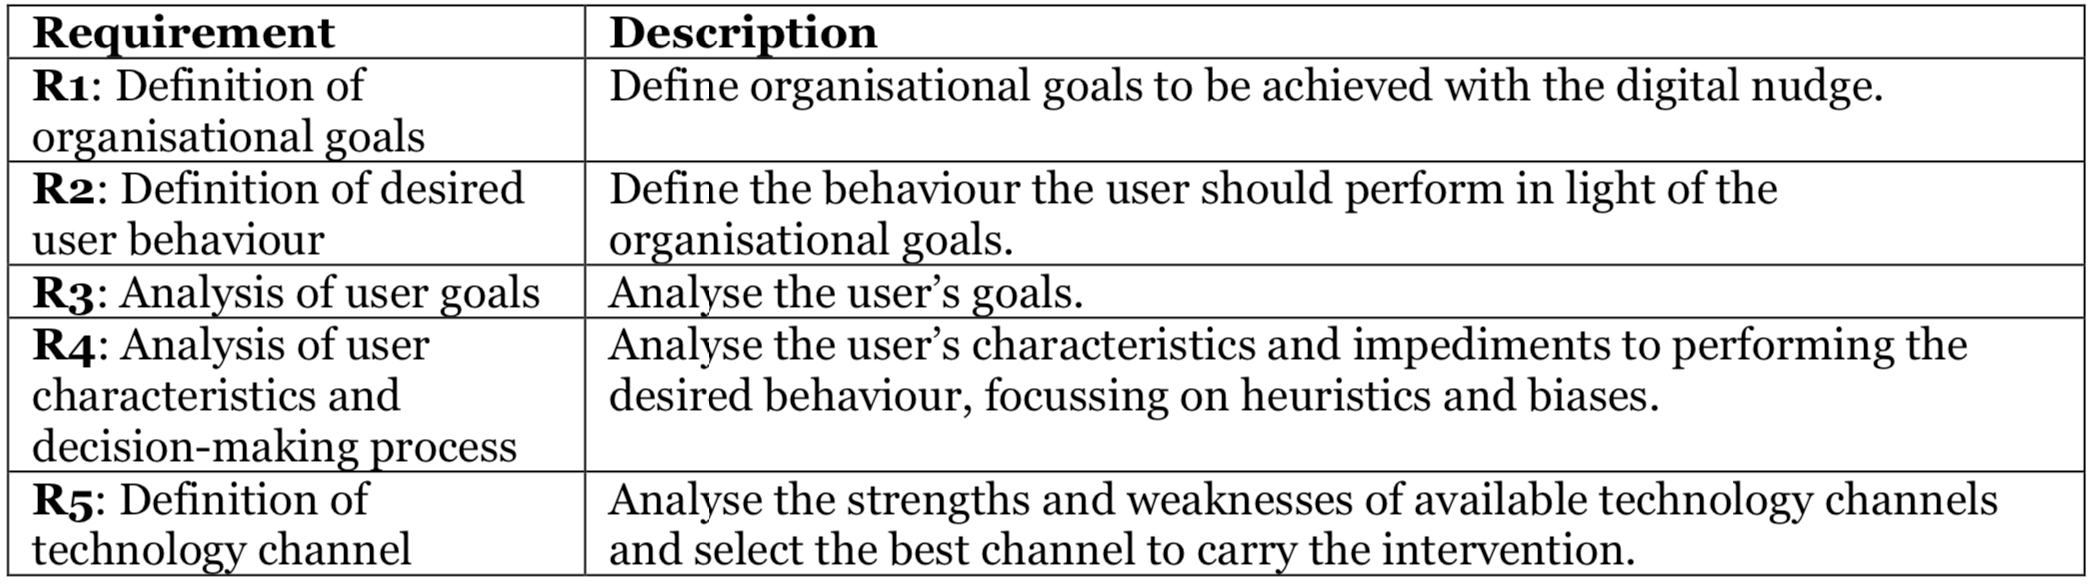
\includegraphics[width=1\textwidth]{images/Phase1.png}
\caption{"Phase 1: Analysing" in Digital Nudge Design method by Mirch et al. \cite{mirsch_making_2018}.}
\end{figure}
\bigbreak

\textbf{ R1:} As the digital nudge intervention was implemented in collaboration with Sats, and their already existing app, this requirement was not applicable. However, we assume that the organizational goals of Sats are to keep members active and aim to help members achieve the national recommendations on physical activity.

\textbf{R2: }The targeted behaviour is regular physical activity. However, we do not aim to measure the effectiveness of the intervention, i.e. whether the targeted behavior is met or not is not the main focus as we rather investigate it qualitatively. 

\textbf{R3:} The users (i.e. the participants)  have different goals, but they share the intention to be physical active at some level. Specifying the different goals is beyond the scope of this task.

\textbf{R4: }Users characteristics varies in age, gender, type of motivation, attitude and interest in physical activity. Identifying all these are also without the scope of this task. (However, some user groups were defined in Chapter 3).

\textbf{R5:} The collaboration with Sats allowed us to nudge users through push notifications in the Sats app. In practise, SMS or email could also be used. 
\bigbreak
\textbf{Phase 2 - Design }
\begin{figure}[h]
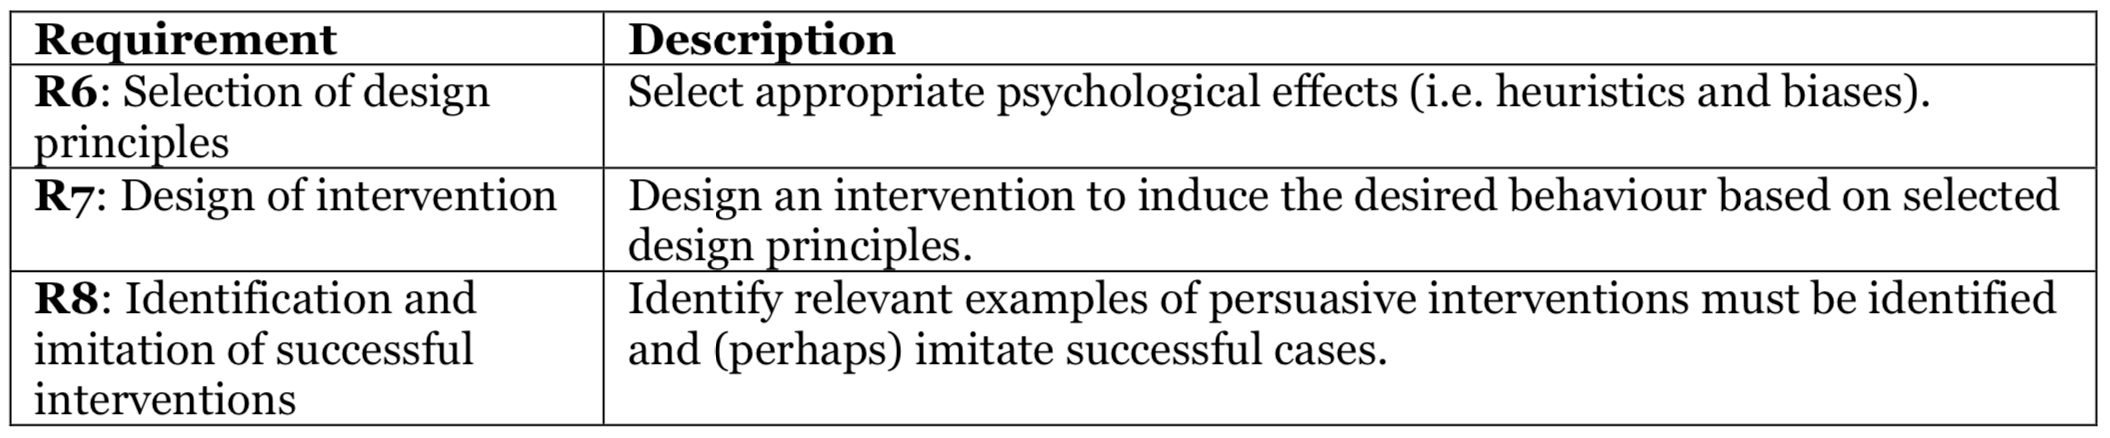
\includegraphics[width=1\textwidth]{images/Phase2.png}
\caption{"Phase 2: Design" in Digital Nudge Design method by Mirch et al. \cite{mirsch_making_2018}.}
\end{figure}
\bigbreak
\textbf{R6:} Message framing was in applied in order to investigate its effect in this context. 

\textbf{R7:} The intervention was designed to disseminate health information that was randomly broadcasted during 30 days. 

\textbf{R8:} The designed intervention was inspired by similar studies of persuasive messages and technologies for physical activity promotion. 
 \bigbreak
\textbf{Phase 3 - Implementation and Evaluation }
\bigbreak
\begin{figure}[ht]
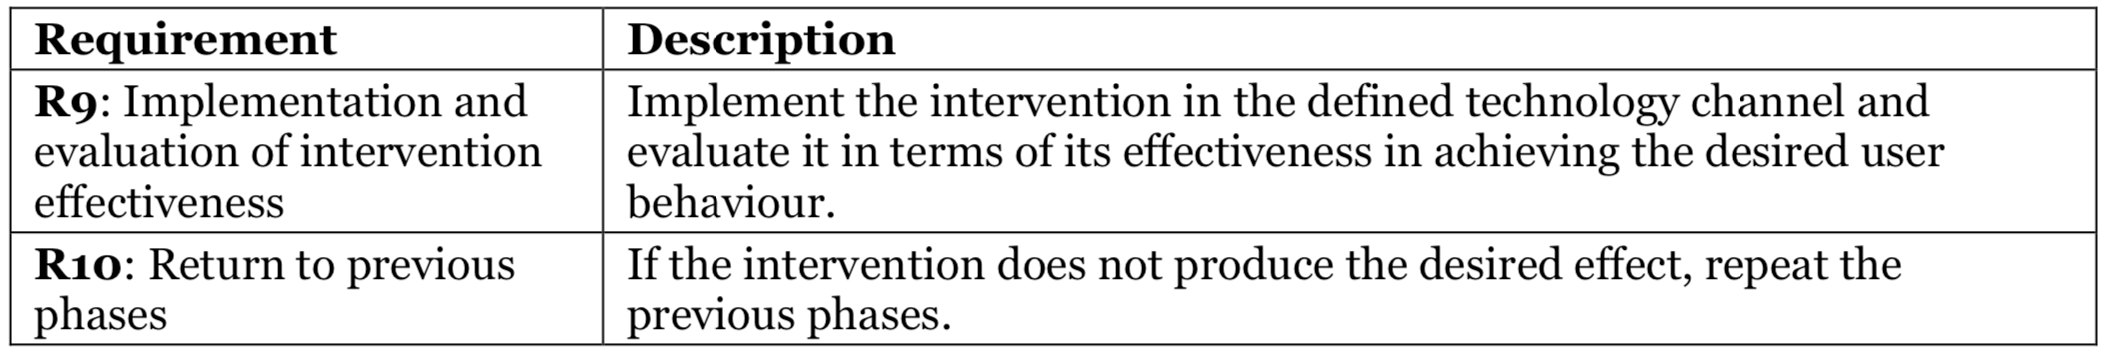
\includegraphics[width=1\textwidth]{images/Phase3.png}
\caption{"Phase 3: Implementation and Evaluation" in Design in Digital Nudge Design method by Mirch et al. \cite{mirsch_making_2018}. }
\end{figure}
\bigbreak
\textbf{R9:} The digital nudge intervention was implemented in the defined technology and evaluated in terms of this research's aims and objectives, i.e. qualitative assessment of users perception and experience. 

\textbf{R10:} As with all other design processes, the DND method suggest that if the digital nudge did not successfully achieve the desired behavior, one should return to the design phase and make adjustments. However this was out of scope for this master thesis. 

\subsection{Content}
The digital nudge intervention was designed to provide health information related to physical activity. Because message framing was applied, it was natural to present positive health effects with physical activity and negative health effects with inactivity. The digital nudges are based on carefully selected information so as not to create commercial and controversial content that could overshadow the perception/experience. The topics were: muscle and skeleton, diabetes type 2, cancer, brain, life expectancy, endorphins and dopamine, mental health and cardiovascular. 

Applying information about health effects coheres with both the objectives of the training center, as they aim to promote physical activity, and the definition of nudging, that should support good choices for individuals best interest. As far as consensus research can gather, physical activity is in the best interest of the individual as well as the society. The presented knowledge is based on multiple reports and expenses from across the world and has been endorsed by international organizations like WHO and national organizations like FHI and Helsedirektoratet. The latter, currently has the leading role of informing Norwegian residents about physical activity. Basing the nudges on such information also contributes to making the information more available, which can be an important step towards reducing inactivity. 

\begin{figure}
    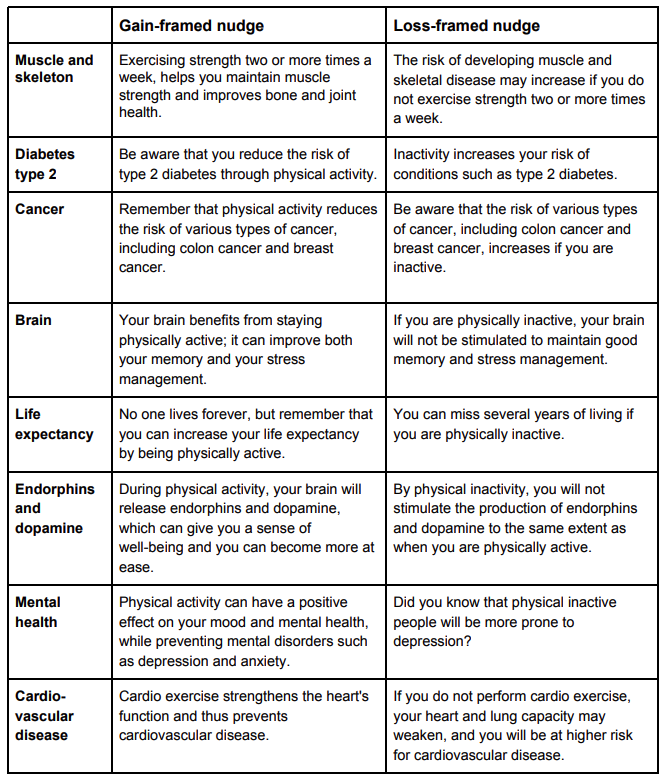
\includegraphics[width=1\textwidth]{images/Nudger.png}
    \caption{Overview of health information that was broadcasted in the digital nudge intervention.}\label{fig:my_label} 
\end{figure}

%\textbf{Tailoring}
\subsection{Tailoring}
%kanskje en del av introduction 
We are aware of the need for tailoring content, and that is also why we are testing this out. We want to gather insight on what should be taken into consideration when tailoring digital nudges. As the review implies, digital nudging is a comprehensive concept, consisting of many design aspects. As the research questions reflects we are approaching how the type of content (RQ1), framing effect (RQ2) and push notification as delivery method (RQ3), affects users perception and experience. 

%People who do not enjoy physical activity will justify the behaviour; Ved å presentere helseffekter kan det skape kognitiv dissonanse. Som vil si at for negative helseeffekter: kan det får en person til å trene fordi de har en intensjon om å ha en sunn helse og ønsker å unngå å ha høyere risiko for å bli syk. Positive helseeffekter: kan få dem som ikke liker å trene til å trene fordi den "rettferdiggjør" en atferd? 

\subsection{Randomization and broadcast plan}
The original plan was that 16 distinct nudges was randomly distributed over a period of 30 days. As timing were not a desired investigation objective, the broadcast of the nudges was randomized, but still within convenient time frames (morning 08-10, noon 12-15, evening 18-20). The original plan for broadcasting can be found in Appendix. Due to Covid-19 only 8 of the intended digital nudges was broadcasted. 

\subsection{Technical implementation}
The nudges were implemented in Sats' own developed CMS (content management system) that allows for publishing content through their app. The CMS communicates with their service platform delivered by Microsoft Azure. Further the service platform communicates with Google Firebase, which provides messaging through cloud, and makes it possible to send notifications to any operating system. Google Firebase connects with users Device ID (users smartphones) and delivers notifications to operating system on their devices. The nudges appeared as push notifications on users locked home screens, but were also presented as a in-app notification when opening the app. 

%"Selve push meldingen (den som operativsystemet gir bruker, og lever på utsiden av appen); Her bruker vi Google Firebase for å kommunisere med telefonen. Den tar utgangspunkt i Device ID (telefonen) og pusher til Device ID eller IDer (om brukeren er registert med flere devicer). Dette oppfattes som selve push-meldingen. Det er vår serviceplattform som kommuniserer med Google Firebase (og CMSet du kjenner til er det som pusher informasjon inn til vår service plattform). Vår service plattform er forresten ren Microsoft Azure."

\bigbreak
\bigbreak
\begin{figure}[ht]
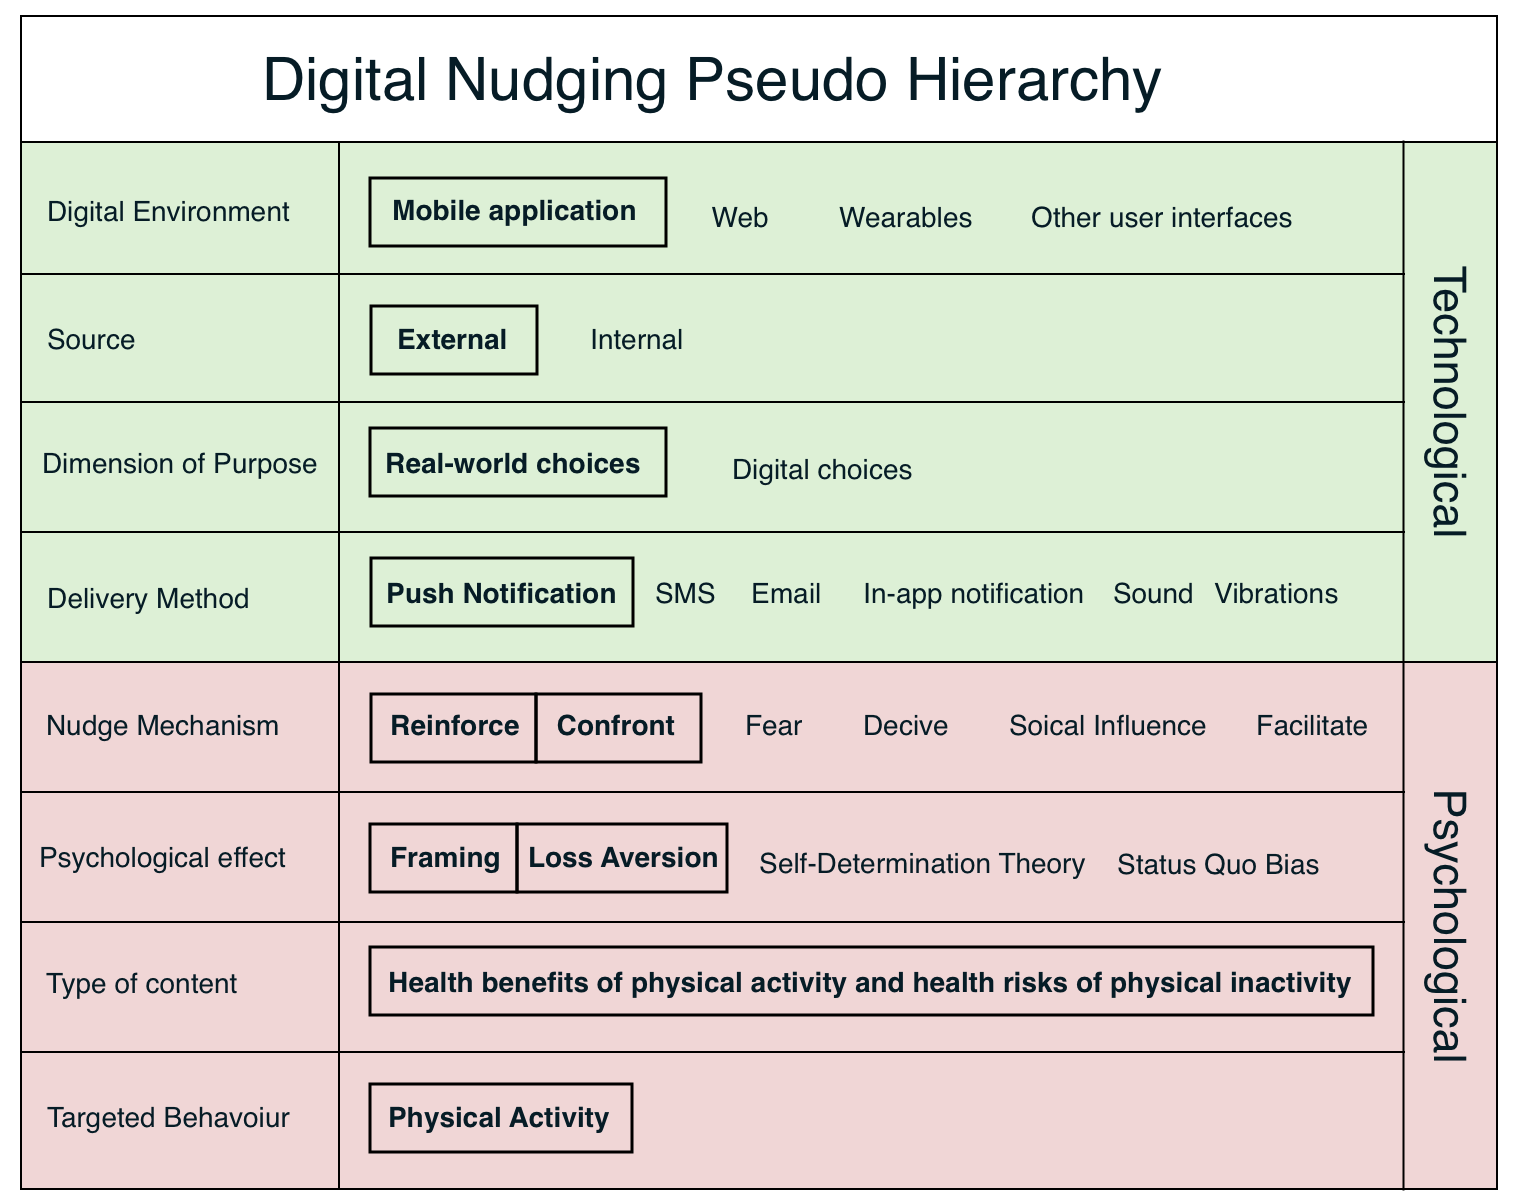
\includegraphics[width=1\textwidth]{images/Nudge.png}
\caption{A delineation of the scope can be illustrated by a pseudo hierarchy that distinguish and sort the terms}
\end{figure}
\bigbreak
\bigbreak

    \chapter{Findings}
This chapter will present obtained data and findings from the thematic analysis, in form of key themes and concepts about users perceptions, that was derived from the thematic analysis, and also present some quantitative data. The themes reflect and represent patterns and prevalence across the data set. 

During the thematic analysis, several categories of perceptions and opinions related to the digital nudging interventions was identified. Various ramifications were identified within the perception and experience of the implemented intervention: no effect (nudge was read but not carefully), minimal effect (nudge was read but not perceived as catchy), encounter effect (nudge was read and perceived as patronizing), incentive effect (nudge is read and provides affirmative effect).

By looking at data about participants perception of the digital nudge intervention, it was identified three main themes:

\section{Theme 1: The Competitive Feed}
This theme embraces the opinions of participants who expressed that they read the nudges to a great extent, but failed to recite the content, i.e. it has not been memorized and the participants accordingly experienced minimal effect. 

%This theme hinges around what happens in the time between receiving and before actually reading the message portrayed by the digital nudges. More specifically , it reflects participants first glimpse and impression of the nudges and what determined if the nudge got attention or not. First step towards influencing choices and behaviors is through the way of communication / contacting / connect / approach : how to reach the target audience ? What attitudes do participants have about push notifications from previously  and how is this mode of delivery perceived in this context? 

\subsection{Attitude towards push notifications}
To understand how participants considered the received nudging we include some of the general attitudes towards the use of push notifications. Many participants expressed how they selectively considered which apps they allowed push notification on. (Note that part of the instructions to the participants were to allow push notifications from Sats specifically, or else it would undermine the purpose.) This was mainly justified by their experience of interference and noise from their phones during the day, which they wanted to reduce as much as possible, i.e. only the most important apps pass through the "allow push notification" filter. Further, general and advance attitudes were that push notifications are easily overlooked in the larger flow of information. 

Furthermore, it appears that people believe push notifications are an appropriate way of communicating content as long as it is perceived as useful. What the participants put in the term “useful” is of course varying; extraordinary messages, news, communication. Even though the addressed digital nudge intervention did not fall under this category based on their attitudes to push notifications, it nevertheless emerged that the vast majority were positive to using push notification to broadcast such information. One of the reasons for this was that general factual knowledge was conveyed and not cliche motivational talk which was associated with exercise/training apps. Also, several participants told that they were interested in physical activity and health in general and therefore considered the nudges as useful. 

Other attitudes towards the general use of push notifications was that if it comes too often, or with irrelevant content, it is perceived as irritating and disruptive. No one expressed that the frequency of nudges bothered or annoyed them, which is good considering that it does not overshadow / color / affect the perception of framing, content and delivery, which is the focus of this task.

Some associated push notifications with commercial content, advertising and not the least social media, and expressed prejudice towards such communications. Others expected it to be information that was urgent and vital and adjusted smartphone settings accordingly. Despite attitudes towards using push notifications to deliver information and regardless of the speculation as to what is urgent or not, they are largely welcomed in this digital nudge intervention, and there were several reasons for that. \textit{“Most push notifications are meant for the other party to profit from it, so I get	skeptical ... associate it with shopping pressure and advertising” (P9)}

\subsection{Easy catching attention}
Despite the overall attitudes and opinions about the use of push notifications in general, it appears that the nudges succeeded in catching participants attention (not every single nudge was given attention, but in the longer run), as everyone replied that they had noticed and read (to different degrees and extents) the push notifications from the Sats app in the given period of time. Participants expressed that whether they gave the nudge further attention after first glimpse, depended on their susceptibility. 

Timing and context were two factors that affected the extent to which the nudge received attention at the time it was broadcasted, i.e. if it was read there and then. Statements included that it was most often not payed attention to at school, at work and in busy situations. In addition, a minor part However, it may also be information (or other UI elements) presented to influence a choice in real-world context, e.g. associated activity meters that remind a user to move (what we will refer to as external digital nudging).  of the participants However, it may also be information (or other UI elements) presented to influence a choice in real-world context, e.g. associated activity meters that remind a user to move (what we will refer to as external digital nudging).  stated that getting push notifications from Sats was downprioritzed.\textit{ "It feels less important that rate that rate reminds me of something" (P8). }

\subsection{The Urgency Hierarchy}
Due to the special circumstances related to the Covid-19 pandemic and the lockdown of the society, a particular opportunity aroused with regards to investigating another category of digital nudging concerning health information. In specific, a SMS was broadcasted to all norwegian citizens on the first day of lockdown by Helsedirektoratet. It contained behavioural advices to limit the spread of diseases, e.g. coffing concerns, social distancing, recommendations on hand hygiene. All participants remembered getting the SMS nudge from Helsedirektoratet. Participants expressed this nudging as more direct and important, and that SMS was perceived as the right delivery method because it was so urgent. 

\subsection{Readability and memorability}

Strong tendency that the nudges were read or partially read by the participants, however the timing for reading was situation dependent. That is, some actually read all while others had read only a few. The nudges were described as short, and easy to read. It required little from the participants in terms of comprehension. It was expressed by several that the nudges maintained participants freedom to read them at an appropriate time, and are therefore not perceived as intrusive. \textit{“It was such a short amount of information that I actually took the time to read it” (P8)}. Everyone claimed to have read the messages to some degree, and more or less all recognized two distinct attributes; 1) Sats, the training center was the sender, 2) There was some kind of health information involved. Further, some participants mentioned topics they remember better than others, i.e. specific conditions or health aspect that were addressed. A more exclusive group, namely one third (1/3) remembered and could recite details about of the different health topics presented. This was predominantly revealed when asking control questions. Statements were:  \textit{"I do not think they have had such a great impact, I have read the information, but did not think much more about it, the information was quickly forgotten" (P4)} and \textit{“When I receive it, I still have the choice to immediately read it or not, which is nice” (P1). }

\section{Theme 2: Food for Thought }
This theme embraces the consistently/common experienced effects of the digital nudging intervention. These findings are important because overall, users' perceptions were that it had some though stimulating effect. Even though these findings are common for the vast majority of participants, there were few strong opinions. 

\subsection{Limited but positive effect }
Participants themselves felt that the nudges had little or no effect on them, in terms of actually making the choice about physical activity after receiving the nudge. Only one participant described how a nudge made him actually go for a longer hike and scheduled a workout the following day. Others mentioned how the nudges planted a feeling that they ought to exercise, but could not answer whether it had actually lead to such outcome.

\textit{"Makes me think that maybe I should go to training today anyway" (P8).}

Still, it appeared that several participants implied that the thought of engaging in some sort of physical activity remained with them during the rest of the day. The extent to which this actually caused them to perform physical activity has not been possible to measure. For example, one participant said that in situations were the idea to workout was present, she would feel more committed to actually complete that workout after receiving a nudge. Further, some participants pointed out that they actually thought about the idea of having a training session (to what extent this was actually done is uncertain), i.e. the incentive was planted. Another participant said that a nudge made her reflect that she should spend an extra hour in training rather than on the couch. 

\subsection{Reminding effect }
The main takeaway concerning the participants perception and experience of the digital nudges, is that it initiated a thought process more than actions and behaviours. In other words, few participants experienced immediate effect, e.g. making a decision about engaging physical activity in the near future or planning a workout. However, the presented health information either aroused deliberate reflection (conscious) or got stuck in the back of their mind for the rest of the day (unconscious). So, even though participants did not decide to go directly to the training center or went for a run, it would stay with them as an consideration whether they should engage in some physical activity during the day. Another important effect of the nudges was that they reminded of the health effects of physical activity. The information about the health effects was already known (to varying degrees), and was also some of the participants justification for physical activity, yet not always in their mind. 

\subsection{Affirmative and infinitesimal motivation}
Another dominating opinion and experience with the digital nudges was that it had an affirmative effect, in the sense that participants got confirmation that their time and effort already spent in engaging in physical activity was worth it. It was a good reminder and support to make them want to continue what they were already doing. Also affirmative in the sense of the information was already known and agreed on, and was used as argumentation to stay physical active. Findings reflect that the digital nudges served as the infinitesimal motivation which had the potential to give the extra push to opt in for  physical activity. 

\textit{“They have served as a confirmation and an extra push that I should continue with what I do” (P15).}

\subsection{Supplementary information and Increased argumentation}
The majority mentions that most of information that was presented was already known, at least to a certain degree. Some of the themes (e.g. cancer) and level of details (e.g. strength workouts should be performed two or more times a week) turned out to be new for several participants. A few participants actually stated that they had expanded their argumentation to stay physically active based on the presented information. 
\textit{"I've added it to the reasoning to keep engaging in physical activity and training" (P9).}

\textbf{Opinions regarding health content} 
\textit{“It makes me think that I'm not only exercise for body and appearance but also for my health” (P3).}
%\textit{“It makes me think I should engage in physical activity based on these arguments as well.” (P3)}

\section{Theme 3: Contrasting Feelings}
As the name implies, there was identifies contrasting feelings among the participants, both regarding the perception of content and framing. 

\subsection{Content}
\subsubsection{Nearby vs. future}
There was a strong tendency among the younger participants (under the age of 30), where several stated distance to many of the presented health effects. They reflected that the information was in fact important, but they displaced it because it felt too far away from their stage in life and distant to make that the argumentation to engaging in physical activity. Typical topics that was displaced by youngers was; cardiovascular diseases, muscle and skeleton and cancer, life expectancy. 
\textit{"I feel that cardiovascular disease and cancer are a bit far away from my concerns" (P11).}
\textit{"The notifications appeal more to the long-term version of myself, and not the here and now version" (P12).}
\textit{"When you are young and healthy, cardiovascular disease feels too far away for making it an argument for engaging in physical activity” (P14).} 
Older participants did not seem to distinguish some topics as less relevant than others. Further, regardless of age, health effects that were easy to relate to and felt close, were perceived as more effective. (i.e. leading to greater potential effect). Such health effects was how physical activity affects the participants "here and now": the brain, stress management, endorphins and dopamine and mental health. 

\subsubsection{Novel vs. familiar}
Older participants (over the age of 30) express that nudges presenting new information was more interesting as they could learn something from it. \textit{"had I been able to learn something from it, it would have been interesting" (P5).}
While other participants thought it was nice and most effective to be reminded of the health effects they had already imposed as an argument for participating in physical activity (i.e. familiar information), as this was not something they were constantly thinking about. 

\subsubsection{Training app expectations}
Another perception regarding content was that participants experienced that the nudges did not encourage any concrete or specific actions, choices or behaviours. The fact that participants had to choose how to use this information, act or respond to it, was experienced as both good and bad. Some participants experienced this as commitmentless, and wanted more concrete information, such as challenges to join, exercises, type of training, etc. Whilst others appreciated the fact that they had the ability to choose how to act on the information. Participants desired freedom of choice and ownership of the choice for engaging in physical activity. 

\subsubsection{Level of appreciation}
A few participants brought up the fact that they had not requested this information to be delivered (expect from signing up  to participate in this research), and claimed that they could take the responsibility of being aware of such information themselves. In other words, they didn't want it since they hadn't asked for it and experienced it as unnecessary and redundant. On the other hand, other participants expressed how it was nice to be reminded, and were happy that the information was provided for them without having to actively look it up. 

\subsection{Framing}
\subsubsection{Strong negative vs. weak positive}
%As we have already mentioned, some participants put limitations on potential effectiveness of the digital nudging intervention. This also involved the effect of different message framings (gain and loss). “It depends on whether I'm in a good or bad period of training. If I had been in a bad period then maybe the other (loss-framed) would have pushed me a little more." (P2)
When participants were asked open questions about what they noticed about the digital nudges they had received, the framing was not mentioned as a property. Due to only receiving 8 nudges, the perceptions, opinions, attitudes and experiences regarding this were vague. Therefore, as an alternative to the intended broadcast schedule, the digital nudges were presented to them in the chat, during the interview. They identified nudges they thought were interesting and received both the gain and loss version of the same message. Without pinpointing the difference in framing, they were asked how they perceived the two versions, and which one that would have greatest effect on them.

%\begin{comment}
\begin{table}[ht]
\begin{center}
\begin{tabular}{|c|c|c|}
\hline
\textbf{Gain} & \textbf{Loss} & \textbf{Indifferent} \\ \hline
15 & 3 & 4 \\ \hline
\end{tabular}
\caption{\label{tab:table-name} Participants categorized by which message framing they experienced as most effective.}
\end{center}
\end{table}
%\end{comment}

\bigbreak
\textbf{Gain-framed}
\bigbreak
A majority of participants experienced gain framed as most effective, because it was perceived as positive, uplifting, rewarding and had a motivational effect. However, their opinions were portrayed in a neutral manner (low voices and engagement), meaning that when they expressed it could have an motivating effect, it was still small. It was also pointed out that it was easier to relate to the positive health effects, especially those regarding nearby topics such as mental health and endorphins and dopamine. 

\textit{“It tells me what physical activity actually gives me, uplifting in style, feels like it rewards me for exercising.” (P2)}

 No participants expressed negative opinions about gain-framed nudges.
\bigbreak
\textbf{Loss-framed}
\bigbreak
A few participants expressed that they considered loss-framed nudges to be more effective due to its serious tone. The perceived negative connotations made a deeper impact on them. 

\textit{“It depends on whether I'm in a good or bad period of training. If I had been in a bad period then maybe the other (loss-framed) would have pushed me a little more." (P2)}
\bigbreak
\textbf{Indifferent}
\bigbreak
Further, a few participants answered that they did not see the gain-framed or loss-framed as more effective than  the other, and argued that other factors, such as content and health topics was more important for their perceived effect. 

%It seemed that people had more opinions about loss-framed than gain-framed. When asked what they thought about the different versions, people often had a lot to say about loss but little to say about gain, yet they claimed that gain had the most effect on them (when it comes to motivating for physical activity).
%The above mentioned findings emerged as we specifically asked them questions regarding their perception on gain and loss (without mentioning or explaining the gain loss term), in order to collect data for the research question (RQ1.a). 

These findings was identified by directly presenting participants with the different framings as it was relevant to the research question (RQ2). However, it turned out that the message framing itself was in fact not noticed by most of the participants themselves, except those who had very negative opinions related to the loss-framed nudges. What turned out was that participants were more opinionated about the varying health effect topics that was presented than the framing.

\subsubsection{Counter effects}
As mentioned, the dominant overall perceived effect is that the nudges act affirmatively on current training and that they act as a push to continue, which shows desirable effects with the implementation. However, when looking more deeper into the impact of message framing in particular, the complete opposite emerges for a few participants. 

Firstly, several participants could identify the negative connotation in the loss-framed nudges when presented side by side. Some of them expressed that presenting the negative effects with not engaging in physical activity was not effective on them because it could lead to bad conscience, scare, warning and felt like they were given a penalty if not staying physically active. \textit{“This one is a little more threatening, warning, tells about the penalty of not exercising.” (P2)}. It was revealed that those who were negative to loss-framed were more committed and clear on what they thought, than those who were positive towards gain-framed. Some did not express any strong opinions, but could still identify the negative framing. And among them, a smaller group of participants expressing rather strong opinions.

On the other hand, negative opinions were expressed about loss-framed nudges in particular. This was the case for a smaller group of participants, but at the same time they expressed stronger opinions (by using more powerful language, several words to describe their opinion, higher voices and seemed to be more engaged than any other participants), and are therefore an important finding. One participants that had strong reaction on it, said that he experienced the loss-framed nudge as patronizing and commanding, which made him demotivated. One participant had extremely negative opinion. The user express that he perceived it as patronizing, a counter effect what we actually want to achieve
\textit{“It feels like I'm being forced to train and yelled at. Such messages does not motivate me to engage in physical activity or workout. To be honest, I am demotivated. The way in which the message is presented makes me tired. It feels like an order and that the push notification knows best.” (P16)}

\begin{comment}
\begin{table}[ht]
\centering
\begin{tabular}{lllll}
\cline{2-4}
\multicolumn{1}{l|}{}                               & \multicolumn{1}{l|}{\textbf{Gain}} & \multicolumn{1}{l|}{\textbf{Loss}} & \multicolumn{1}{l|}{\textbf{None}} &  \\ \cline{1-4}
\multicolumn{1}{|l|}{\textbf{Extrinsic motivation}} & \multicolumn{1}{c|}{10}            & \multicolumn{1}{c|}{2} & \multicolumn{1}{c|}{1} &  \\ \cline{1-4}\multicolumn{1}{|l|}{\textbf{Intrinsic motivation}} & \multicolumn{1}{c|}{5} & \multicolumn{1}{c|}{1} & \multicolumn{1}{c|}{3} &  \\ \cline{1-4}
&&&& 
\end{tabular}
\caption{\label: Shows how many participants preferred the different wording of the message.}
\end{table}
\end{comment}

\section{Theme 4: HVOR SKAL RESTEN}

\subsection{Susceptibility factors}
As the data indicates, the digital nudges are read because of its readability and effortlessness, but what happens next depends on…Susceptibility factors affects participants perception of the message, and thus further determines whether the information is considered and reflected on (?). Susceptibility refers to participants likelihood to absorb and reflect on the presented information. While and after reading the nudges, several factors impacted participants susceptibility, i.e. their further choice (unconscious and conscious) of acting, responding, or reflecting, on provided information. Our findings suggest three categorizations; 1) timing, 2) content-dependency (meaning that the perception of nudges is content-dependent) and 3) personal characteristics/psychological effects. 

\subsubsection{Hvor skal denne: Timing}
Timing and context has already been mentioned as a factor to determine if the nudge receive attention or not. After read, the timing and context still has influence. Although a participant defied poor timing and context when receiving the nudge by reading the nudge, this assessment continues into how they respond further. That is, timing and context are two-way / two-layer barrier. \textit{“I think that could ever come back to what I haven't had time to reflect on, it's going to be a bit like the defense in everything about information, you register it, also disappear” (P8).}

\textbf{Source Credibility vs. trustworthy information }
Regarding credibility, the vast majority agreed that they could rely on the information that was conveyed. Some justified it because it was common knowledge that they already knew to some degree. Others pointed out that since it came from such a big player as Sats, they trusted the content. This was revealed through direct questions. 
“I find the information very trustworthy since it comes from Sats which I believe is the largest fitness center chain in Norway, it never struck me that I should be critical to the information” (P12)
“I do not doubt the information even if it comes from a commercial operator, I trust the information that is sent ” (P11)

\textbf{Conditional effect}
In addition, several participants described how the nudges could have been effective or more effective given this or that condition. This is mentioned both regarding the nudging in general, but also directed specific towards the message framing. Typical conditions that affected their perceived effect are: current training routine, prior physical activities frequency, work situation and free time, prioritizations, timing, lack of motivation. Some of the statements were: 
"If I had not trained normally and would be positively influenced to exercise, I think that is the kind of information I would like to be notified of ” (P22)
"The periods when I work a lot of overtime it is a little more demanding to get into training, if I had received one of the alerts in such a situation it might have influenced me to go  training anyway" (P19)
"If I had gotten them at the right time, e.g. the days I am struggling to get to workouts, they might have had a bigger impact on me" (P18)
“It depends on whether I'm in a good or bad period of training. If I had been in a bad period then maybe the other (loss-framed) would have pushed me a little more." (P2)
These are augmentations are only hypothetical, meaning that it is not the current experience with the nudges. Makes it weaker than the answers where they do not express conditions to their answer. This is a group that shows how content awareness is important.

trust/urgency source credibility/delivery channel hierarchy and 


















    \chapter{Discussion}
This chapter expand on and discuss the presented findings, compare it with the reviewed literature and state its relevance to the research questions. The research objectives was to…. explore users experience and perception of the digital nudge trial, and gain information about how aspects like framing and delivery method affects the perception and experience. 

By answering the RQs we are able to gather insights that could be used when tailoring digital nudge interventions in the future. 

\section{Overskrift?}

\subsection{Automatic vs. reflective processing}
Caraban et al. \cite{caraban_23_2019} stated that the automatic systems should be further exploited when it comes to technology for influencing behaviour, as most of our choices are made by this system, however few studies seem to approach it. The choice to engage in physical activity, such as workout or take a walk is usually not an automatic choice as it is conceivable that for many people physical activity is perceived as more time-consuming behavior than, for example, remember to use dental floss or wash your hands properly. This means that this behavior often requires planning before the implementation can actually happen. However, when physical activity becomes a habit, the choices are made more automatically (people have a knack for acquiring routines). This means that the choice of physical activity can be a result of both automatic processing (I go to training today because I do every Monday) and reflective processing (I go to training today because it's good for me). It seems that the implemented nudge intervention tap onto both the automatic system (when the push notification catches attention and is read) and the reflective system (when participants reflects on the presented information). However, it is only when the reflective systems is touched that the nudge seem to have a positive effect(?).But what our findings indicate may be that for receive users attention, we approach the automatic system, though the push notification. And this could mean?

\subsection{Educational effect}
One would believe that most people are aware of the conveyed health information information as it is consensus and not high level knowledge, and obtained from actors such as WHO, FHI and Helsedir. Our findings show that some of the information (especially regarding cancer) was new to the participants. The fact that some participants actually said they had expanded their reasoning and motivation to be physically active suggests that it has an educational effect. Norwegian citizens know a lot (as most of the consensus information was recognized) but there is still a lot of information that has not reached everyone yet. The digital nudging may not have had an immediate effect on choices and behaviors as such, but it did have an effect on attitudes and knowledge, which often underlies behavior. Further, this proves that there is a need to make information from such actors more accessible, for instance through digital nudging (related to mobile apps). 

\subsection{Technology channel/delivery method}
It is known that the first step in persuasion is getting users attention, which could be inherited to digital nudges in the form of signals as well. The DND method \cite{mirsch_making_2018} suggest choosing an appropriate technology channel, but there is a lack of research on which channels are most beneficial for different types of nudging.  All we know is that there are many to choose from. We chose to implement digital nudging through push notification because it was an easily accessible feature and because it ensures that as many as possible are reached without seeming intrusive. Our findings confirm this assumption?? Furthermore, it was interesting to compare it with other delivery methods, e.g. Helsedir SMS nudging. 

\subsection{Covid-19 Nudging: communication channel and source credibility}
As stated in Chapter 5, the covid-19 pandemic gave us the opportunity to compare our nudging intervention with a recent case of governmental use of nudging. Helsedirektoratets nudging did not address physical activity promotion, but it conveyed other types of recommendations on behavior related to public health, more specifically regarding infection control. The two are similar considering that they both promote health preventive behaviors, and are virtually based on the same source (as the health information in Sats intervention was endorsed by Helsedirektoratet and FHI). The main difference is that the information was broadcasted through different channels, and our findings indicates that they are perceived differently in regards of attention, commitment and severity/urgency. Utilizing a more personal communication channel, SMS was experienced as more direct than push notification, with the intention that is was read and absorbed more or less instantly by all receivers. Participants told that they almost felt like a civic duty. There was no room for reactions other than to follow the recommendations, i.e. they felt commitment to engaging in the behaviour. Whereas the push notifications also felt like receiving recommendations, they expressed that it was up to each individual to figure out how to respond or act on it. 

Further, it seems that SMS has greater certainty of reaching the user, as push notifications often get lost in the information flow. Push notification captures the user's attention and is read at some point, but the information is not experienced as seriously as the SMS from Helsedir. 

What is more important; the message itself or the communication channel? It seems that the choice of channel could have greater impact than the actual content. 

How would it be perceived if Helsedir sent health information about inert (?) and slow moving disease, motivated by the gap between recommended activity levels and the actual activity levels. Could it be that such communication could obscure and dilute more urgent messages? Would the public approve of it? And would it strengthen the sense of commitment if Sats had actually stated that the information was advices from public actors such as the Helsedir. 

These findings indicates how the sender or source is crucial for perception of message. This can be compared to the work by authors X \cite{oinas-kukkonen_persuasive_2009} (Reference: Persuasive Systems Design: Key Issues, Process Model, and System Features) where it is stated that the credibility is an important property of a system aiming to persuade the user about a behaviour. The sender of the nudges (i.e. Sats) is perceived as trustworthy and domain expert by most of participants. However, Helsedir is perceived as trustworthy to an even greater extent and therefore has greater influence. It is conceivable that the perception of seriousness and sense of commitment would be strengthened if it was stated that the information originally comes from Helsedir. 

\subsection{Gain vs. loss}
Our findings indicate that in the context of physical activity promotion amongst gym-members, gain-framed nudges are perceived as more effective than loss-framed nudges. This is consistent with previous literature on message framing in other physical activity related context and the prospect theory. 

Further it was also found that the participants had stronger emotions regarding the loss-framed nudge, than gain-framed, which is consistent with the loss aversion theory ????? (Reference). 

\subsection{Ethics of nudging}
The fact that the participants understood the intention of nudging and that they felt that their freedom of choice was maintained proves that the implemented intervention is in line with the nudging requirements.

\subsection{Psychological effects}
Biases and heuristics are depend on each other, hence it was not just the framing effect that emerged through the findings. From Self-determination theory we know that humans are in need of feeling autonomy in the context of exercising behavior. I.e. if technology aiming to influence decision-making could imitate that feeling it is more likely to be successful and achieve that choice or behaviour. Our findings show that participants experience the choice of engaging in physical activity to be truly their own, even though they were exposed to external influences. 

It seems that participants that expressed that loss-framed nudges was most effective felt cognitive dissonance; they are a member of the gym with an intention to have good health. When negative effects are presented people will do everything to ensure that this does not apply to them, because that would feel uncomfortable when they in fact have the intention to be at good health. 

\subsection{Minimal Effect}
Some participants pointed out that they did not think the digital nudging had any effect on them (does not mean that they experienced it negatively, but more indifferent). One of the reasons for this could be because they considered the effect to be an immediate action or choice regarding workout after receiving the nudge. Hence, as they did not decide to or plan a workout immediately after reading the message they concluded that there was no effect. However, the aim to influence people's choices regarding behaviour should more be seen as a process than a single choice and its effect. This means that such interventions need to be investigated over a long period of time in order to say something about the real effect. As we wanted to understand how the intervention was perceived, effect was not limited to the degree of achieved immediate behavior, i.e. that the nudge led to a workout or not. This should probably have been made clearer during the interview. (it doesn't need to be a workout at Sats, all kind of physical activity is good).

\subsection{When nudges fail: Counter effects}
Caraban et al. \cite{caraban_23_2019} made us aware of the possibility of negative effects of nudging, and emphasize how this should be taken into account in understanding how we can design effective nudges. Our findings show that some nudges led to counter effects for a minor part of the participants. In particular, the loss-framed nudges were experienced as patronizing, and hence demotivating, for some participants. This implies that some nudges actually leads to the opposite of desired behaviour. Others viewed the nudge intervention as a whole as moralizing and provocative, considering its content as the focus on illnesses and disorders. There was apparently no connection (no common characteristics) between the users that voiced the digital nudging intervention as a whole and those who voiced loss-framed nudges, as impacting in a negative way. What these participants had in common was that they did not exercise for their health, they trained because it was fun (expect the guy that was demotivated, he was not interested in training at all). This is not at all favorable, and needs to be considered for future applications. Previous quantitative studies have not been able to detect such effects, which implies the importance of this qualitative assessment.  

\section{RQ1: How are digital nudges based on consensus health information, experienced and perceived by gym members?}

The study shows two distinct directions among participants / gym members perception and experience of the intervention. 

A larger group of participants experienced positive effect in the form of reminding, affirmative and uplifting. 


On the other hand, a smaller group of participants felt that it was moralizing to communicate health information in this way. These participants had particular opinions about the loss-framed nudges. 

However, we found no apparent correlation in personal characteristics between the participants who expressed the different paths, and further studies on more specific user groups among this target population must be done in order to establish more concrete guidelines for tailoring. 

\section{RQ2: How does message framing affect users perception of the digital nudge?}

It should be said that the basis for exploring message framing was amputated with regard to Covid-19, so the features are few and weak.

There has been a lot of focus on message framing up over the years with persuasive research to influence behavior such as physical activity. It has been pointed out that the framing of a message has great impact.  

Strong and negative opinions about loss-framed nudges were expressed, while neutral (and positive) opinions about gain-framed. Even though this only holds for a minor part of the participants, this points out that using the wrong framing can have a greater negative effect than the effect that comes from using the framing correctly. I.e. when applying message framing to digital nudging or similar persuasive interventions, it is crucial to avoid using wrong framing. To be on the safe side, practitioners implementing digital nudge interventions should therefore frame their message from gain perspective, until otherwise is proven.  We also tried to find correlations between users characteristics (defined user groups) in regards of preferred message framing, but did not find any of significance. 

Greater impact in the negative direction if incorrect framing is used, than impact in the right direction, i.e. message framing is not the ..

On the other side, it was found that message framing did not affect users perception of digital nudge intervention to great extent, and other factors seemed to be of greater impact. 


\section{RQ3: How are push notifications experienced as the channel for broadcasting digital nudges?}

Push notifications are experienced as a suitable way of digital nudging. 
Push notifications makes information available / easily accessible but also easy ignorable (hence does not interuptive)  
Effortless but also commitmentless (due to content)

The nudges could in principle be broadcasted in different ways, for instance through SMS, email or in app notification. The advantage of push notifications is that they are widely read, compared to eg mail.

Furthermore, it appears that the sender plays a role in users perceiving the information as credible.

\section{Limitations}
There are some limitations regarding this study that needs to be addressed.

\subsection{Changes and adjustments in regards of Covid-19 }
The plan was to broadcast the digital nudge intervention over a 30 day period, which is originally very short in terms of influencing behavior. Due to the covid-19 pandemic it was not possible to complete the intervention, and only 8/16 nudges were sent out. This makes the basis to test holistic health information limited and it is difficult to spot standout nudges. Further, this weakens the findings, and additional research needs to be conducted in order to confirm the preliminary findings of this study. There is also a educational aspect - For instance we found that the conveyed holistic health information, most of it was known from before but something proves to be new. By testing the nudging intervention over a longer period of time (preferably over several months) one would gain a better understanding of what information is catching, being remembered, new, etc for the participants. The holistic picture of this is needed to say something specific about tailoring digital nudges. 

It is also conceivable that doing both pre and post interviews would strengthen the understanding, as we could see how attitudes, knowledge, intentions, motivation and behavior change after the intervention. Similarly, quantitative data can help to understand the bigger picture.

This also led to some of our findings not being based on real-world perception and experience anyway, as we had to present some of the nudges during the interview.

To adapt to the circumstances and still be able to answer the research questions,, we chose to present some of the nudges during the interview. This also led to some of our findings (especially those concerning framing) not being based on real-world perception and experience, as first intended. 

\subsection{Sample selection / Variations across participants}
As it was an exploratory research we found it okay to invest a bigger group. This was also done in regards of convenience sampling. However it turned out that many persons wanted to participate in the study, and we could have been more selective when scheduled interviews. 

Due to this, there is a variation across characteristics such as age, motivation type, prior physical activity level/habits, etc. 

To be on the safe side, we gathered quantitative data about participants in order to be able to define groups within the sample, but we did not see any connections / correlations between the characteristics (in addition it turned out to be out of scope for this thesis). 
Due to time constrictions, corona and ethics of doing research we used convenience sampling. As we imposed convenience sampling for this study, the 
Among those who signed up as participants in the study, the selection was representative. But due to the time constrictions (lost time due to corona) we had to make interviews with the ones available first. We did not have time to sort of age and gender, even though we had the opportunity for it in regards of number of participants and the variation in age and gender. The time limitations was one of the consequences of corona pandemic. 

The intention to include training members was that among this group / selection of people there will always be someone who trains a lot and someone that does not, meaning / in other words; it was representative for a large part of Norway's population. However, all members of training center share / has one ting in common; the motivation / intention to engage in some form of physical activity, because they already became a member (invest money in their own health). When we consider Fogg's behaviour model, we see that motivation is one of three fundamental elements that needs to be in place for a behaviour to occur. Ability and prompts are the other two. 

\subsection{Definitions and interpretations }
During the interview we clearly stated how we defined physical activity, ie.e that it did not have to concern a workout at Sats. However, participants often tend to use the term workout or training. For instance “It did not motivate me to workout”. Which makes some of the details about the data somewhat ambiguous. This is something I should have made clearer during the interview: it doesn't need to be a workout at Sats, all kind of physical activity is good.
The same regards the term perceived effect, which can be defined in many ways. The question regarding their perceived effects was open and without restrictions, in order to capture the different types of real and honest effect.



    \chapter{Conclusion} 
%Final remarks, concluding thoughts, and suggestions for further research.

\section{Final remarks}

\section{Concluding thoughts}
This study aimed at investigating how a digital nudge intervention for physical activity promotion was received, perceived and experienced by users at a gym-center. By doing this, we gathered insights which contributes to the bigger question on how to nudge.

Ble heller en generell innnsiktsamling på hvordan oppleveseln av slike nudger er og potensiale. 

Generelt sett har vi samlet masse innsikt på hvordan digital nudging burde bli implementert for fsysisk aktivtet. Dette er første steg mot å forstå mer om hvordan vi kan designe effektive nudger for denne konteksten. 

Ved å inkludere brukere og kvalitative data har vi greid å ... 

Nyttig innsikt har blitt avslørt ved å se på message framing in the context of digital nudging, 

Det kan tenkes at dette er et funn som kan gjelde for andre persuasive technologier også, men det kreves videre forskning for å bekrefte dette. 

What did we find out:
- Gain is preferred 
- Using push notification as the method for delivery has both strength and weaks, more interaction and commitment could make it more promising
- Examples of Self-determination theory appeared in the study, indicating that this should be taken into consideration for next implementations
- Dette er en lovende bruk at digitale nudger (så lenge du ikke bruker loss på folk som ikke vil ha det)
- Som vi allerede vet er timing og context viktig, 
- Other types of content, more concrete and suggesting etc (facilitator)

Findings suggest that commitment 

By doing a qualitative assessment of the digital nudging intervention, we obtained some opinions that do not appear in a quantitative study. For example, we have found that loss-framed can cause negative / opposite effects for some users, which is highly undesirable. 

For å si noe mer spesifikt om tailoring, må det også gjøres bedre kategoriseringer på folk på treningssenter. 

By making a qualitative assessment of the nudging intervention, we obtain some opinions that do not appear in a quantitative study. For example, we have found that loss-framed can cause negative effects for some users

\section{Further research}
Ut fra funnene ser vi at det kan være interresant å benytte seg av annen type nudging enn (signal). Facilitator burde bli undersøkt ettersom brukere understerker at de trenger noe mer konkret, ikke bare helseinformasjon. 
Det ville også være interresant å kombinere informasjonen med forslag, for å oppmuntre til både interaksjon med appen. Direkte kommunkasjon. gjøre dette - kommando. 

Annet type innhold, annen leveranse, annen mekanisme og bygge på andre biases og heuristics. 
Sammenligne ulike implementeringer for å finne ut hva som er det beste for denne konteksten. 

Future research should continue to test and evaluate various digital nudging implementations in real-world context, so that we can increase our knowledge of how to nudge through digital environments. As well as how we can make the best use of technology and human psychology to help and support good choices in relation to health. 

Digital nudging involves many components; mechanisms, what psychological effects should we utilize, delivery methods etc that work best for the given context. This study was the first attempt to evaluate a digital nudge intervention based on qualitative data, and has contributed a lot of new insights that cannot be revealed with quantitative studies.

It would be interesting to do similar user experience studies concerning other types of digital nudges, to get a insights from the users perspectives. Of course, it could strengthen the findings if the study was rearranged but with controlled user groups, including both inactive and active participants.   

Researchers should continue to do qualitative studies around users' experiences and perceptions of various digital nudge implementations. 

By applying the framing effect to digital nudging for physical activity we also saw other psychological effects... 

There is a need to explore other psychological effects that can be applied in digital nudging interventions, to make them more effective.

In future, researchers should use the design frameworks and guidelines, in order to implement digital nudge interventions, 

%Hva hvis våre helsenudger hadde blitt broadcasted til hele norges befolkning? vi antar det ville blitt oppfatte i det negative leiet. 


\subsection{Long-term effects}
It is known that studies regarding the long term effects is low for many HCI topics, including digital nudging. It would be extremely interesting to study this context in longer time interval, to see if this informational nudges had an impact over time. One of the participants actually expressed that "maybe over time, it would have a stronger effect on me". 
    
   % \bibliographystyle{plain}
    \bibliographystyle{ieeetr}
	\bibliography{references}
    
    \appendix
    \chapter{Appendix}
    \chapter{Appendix}

%\section{Appendix A: Interview Guide}
%\section{Appendix B: Information sheet + Consent Form}
%\section{Appendix C: NSD Approval}

\begin{figure}
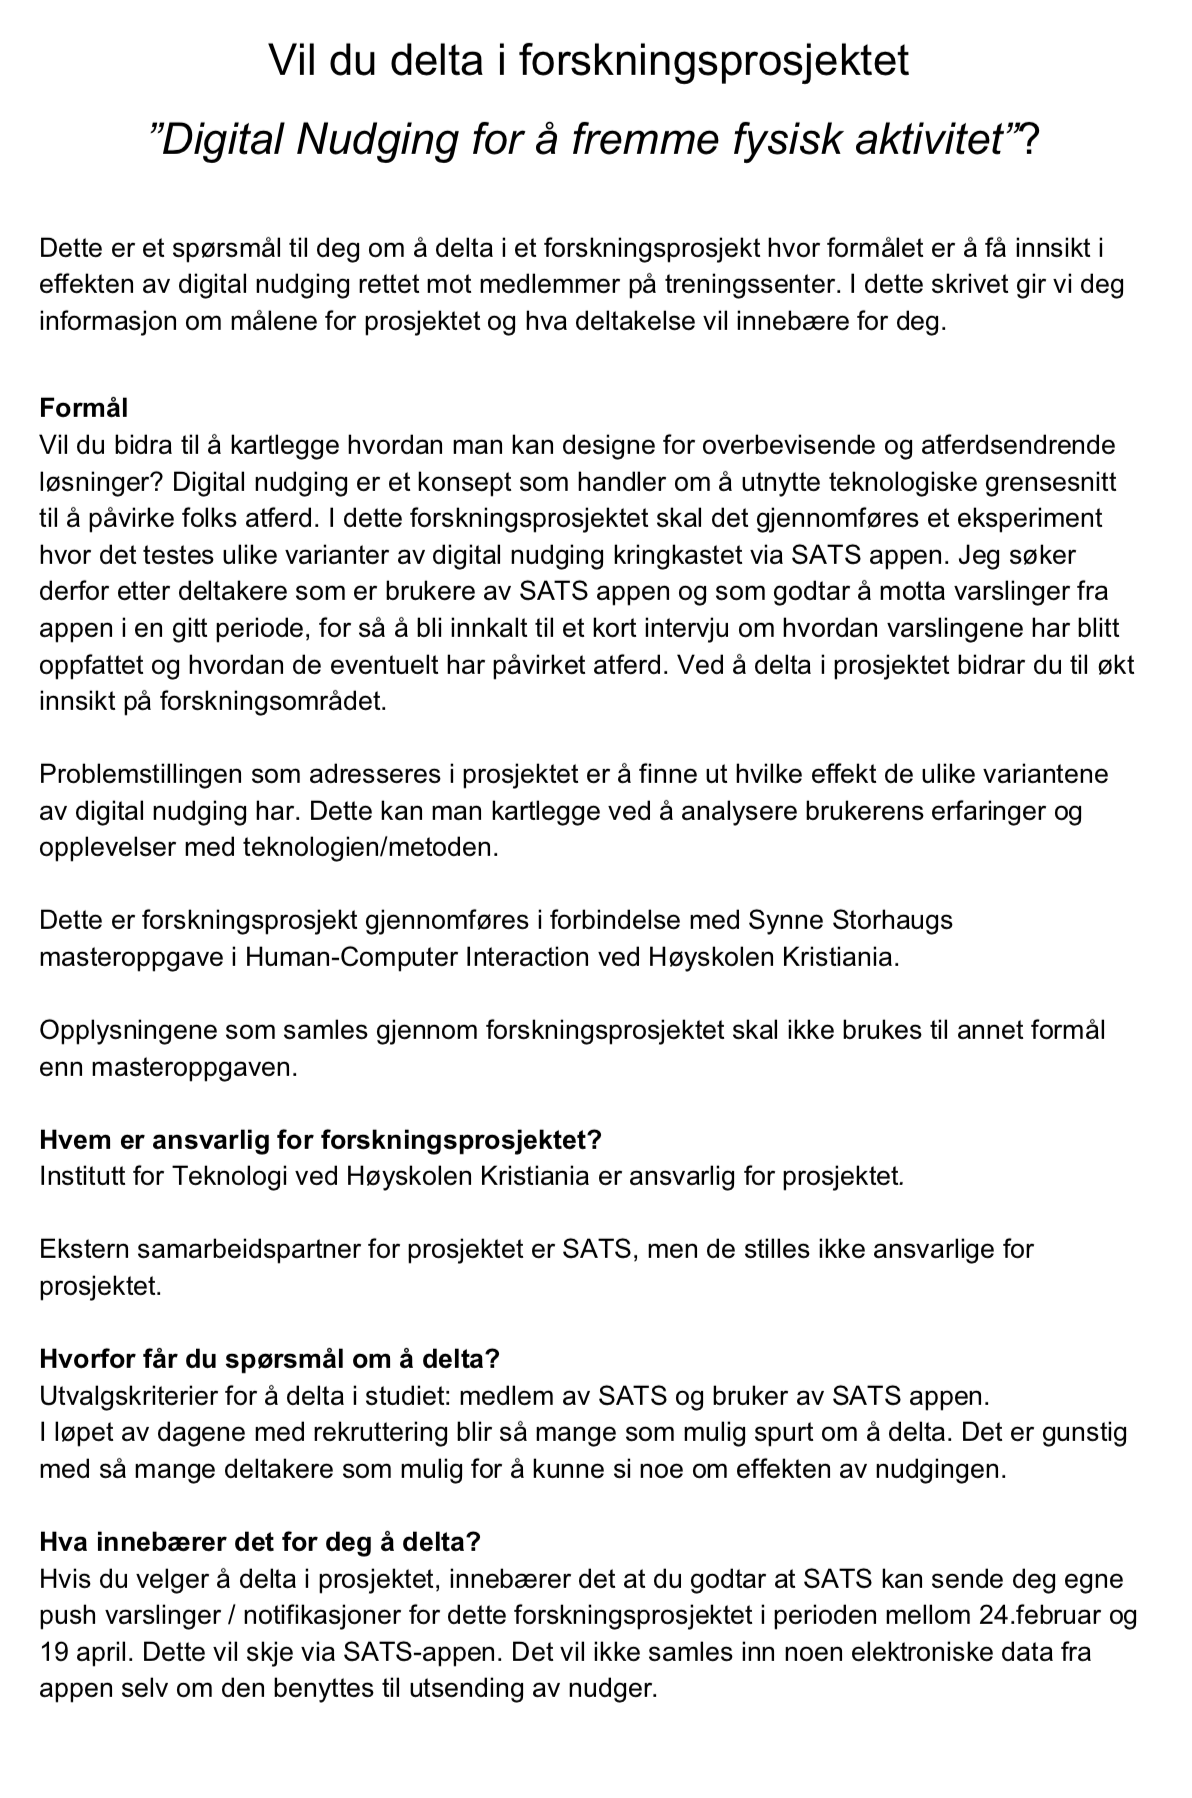
\includegraphics[width=1\textwidth]{Side1.png}
\end{figure}

\begin{figure}
    \centering
    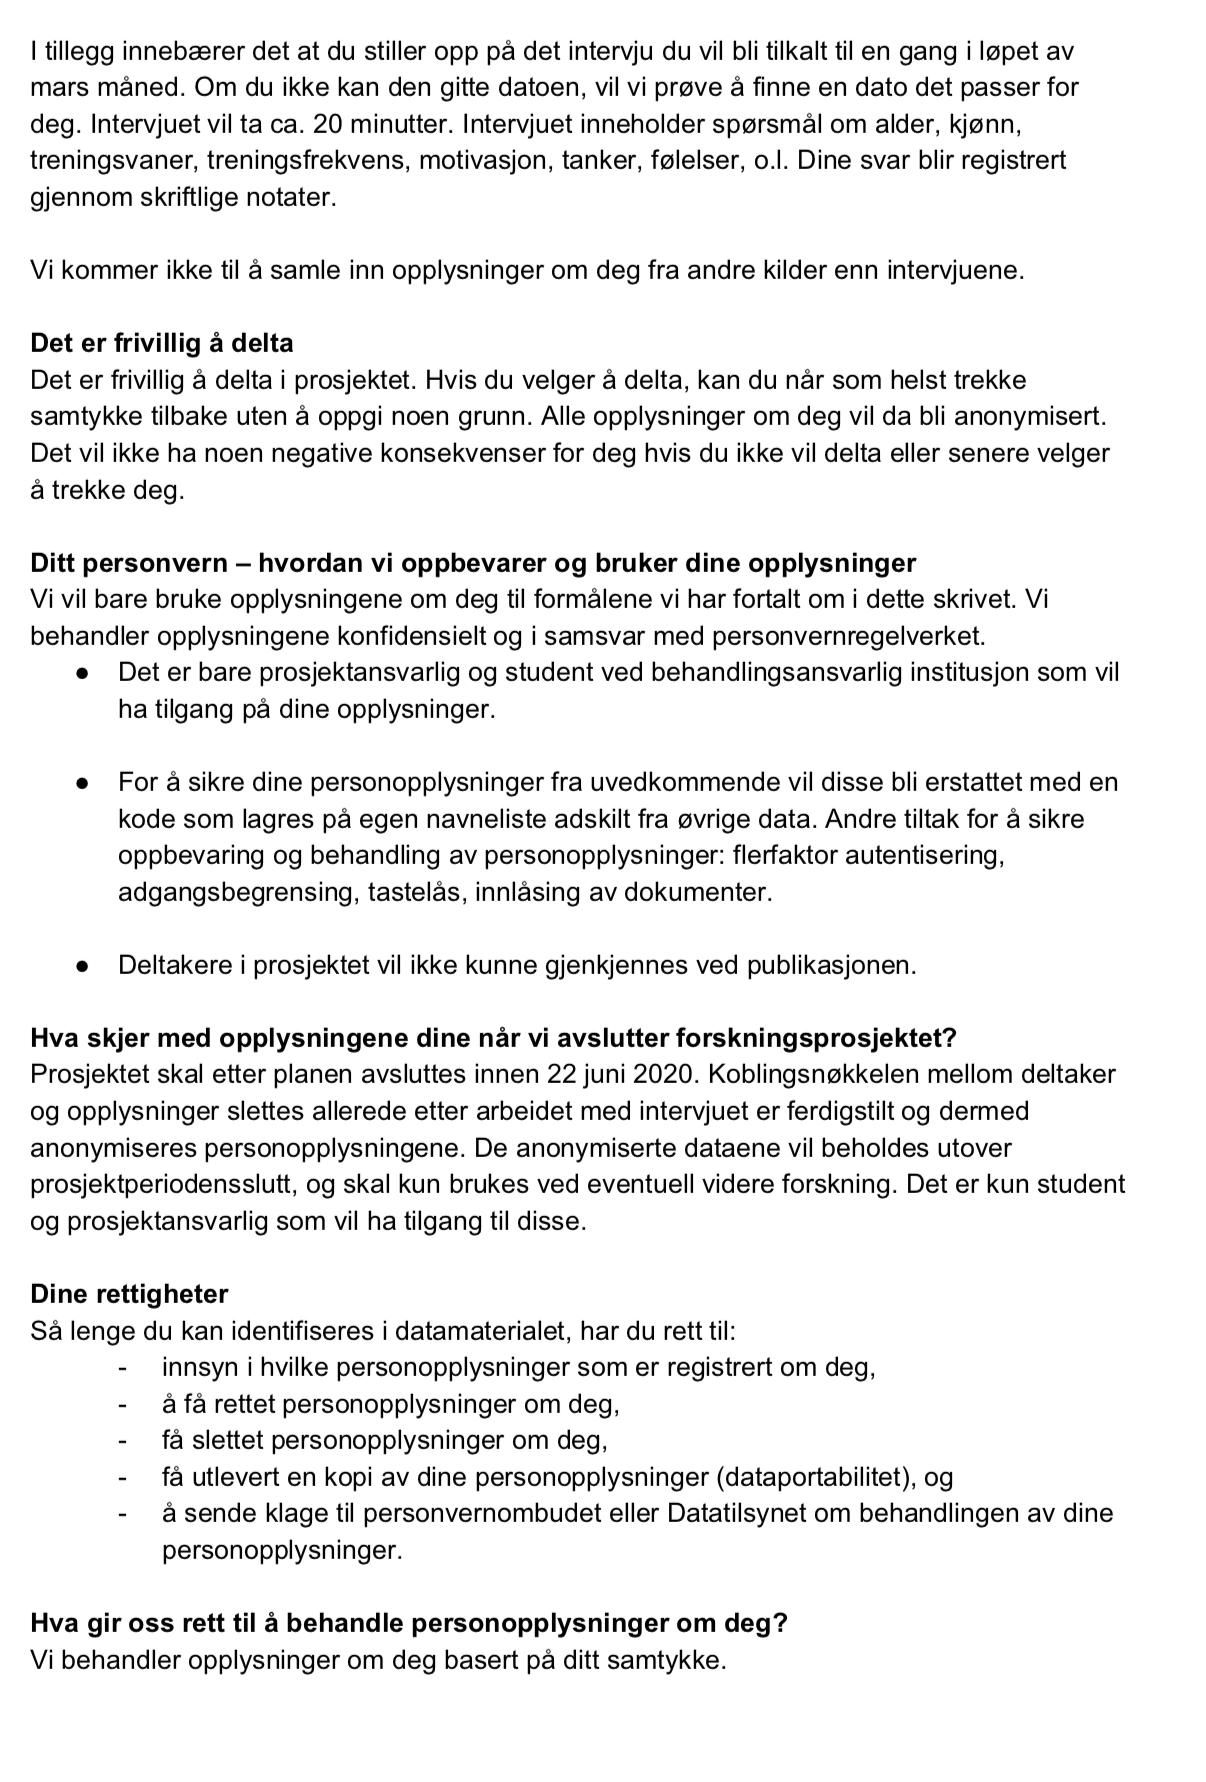
\includegraphics[width=1\textwidth]{Side2.png}
\end{figure}

\begin{figure}
    \centering
    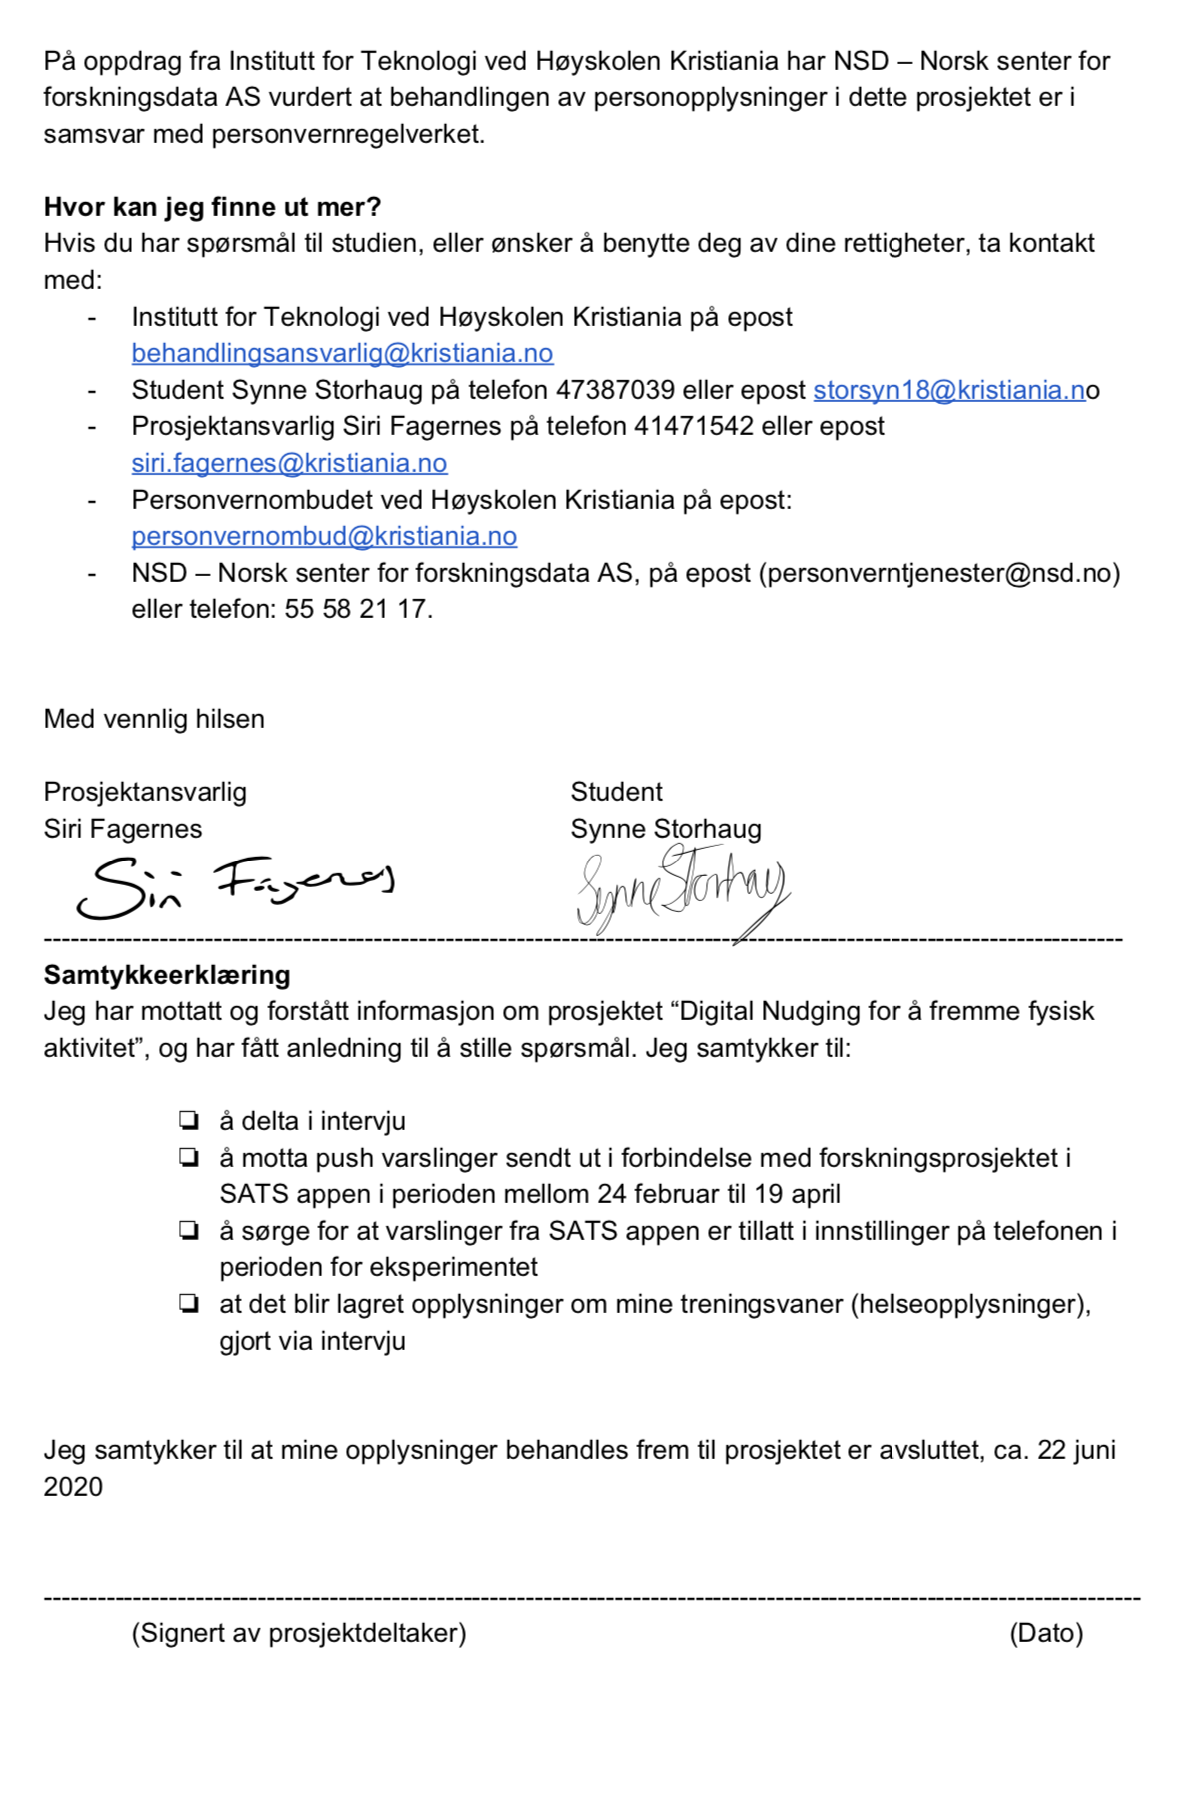
\includegraphics[width=1\textwidth]{Side3.png}
\end{figure}

%\begin{figure}
    \centering
    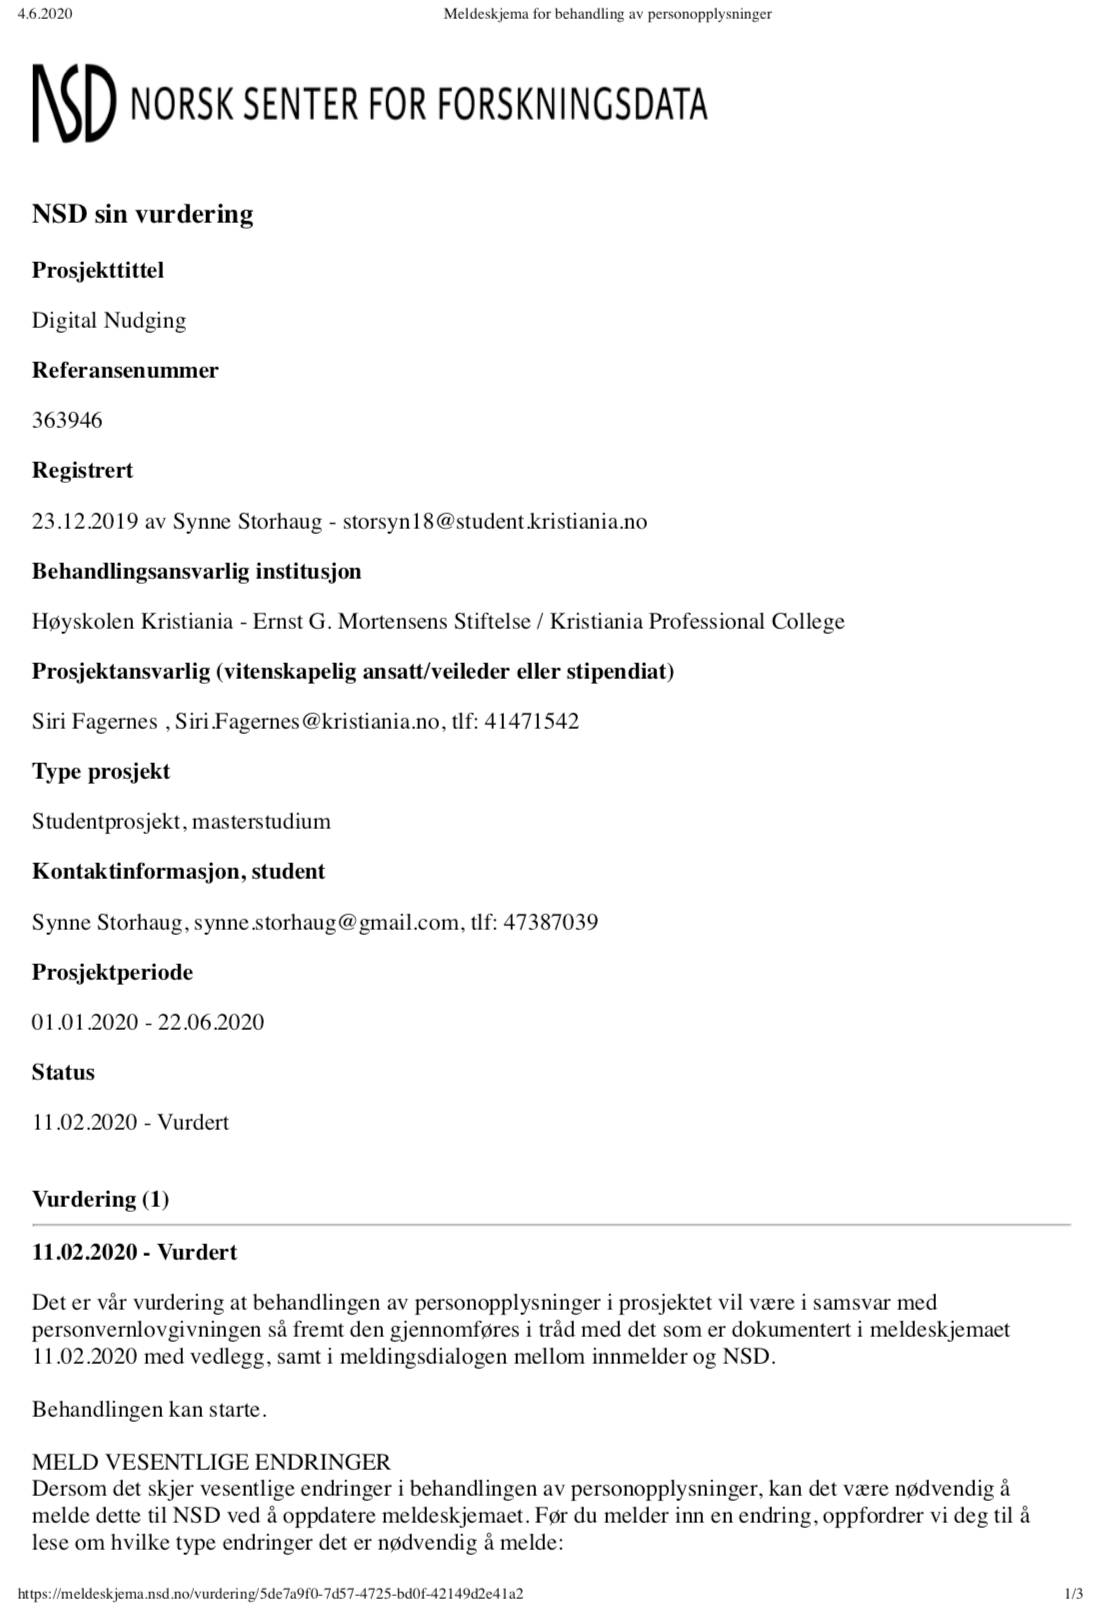
\includegraphics[width=1\textwidth]{images/MS1.png}
%\end{figure}

\begin{figure}
    \centering
    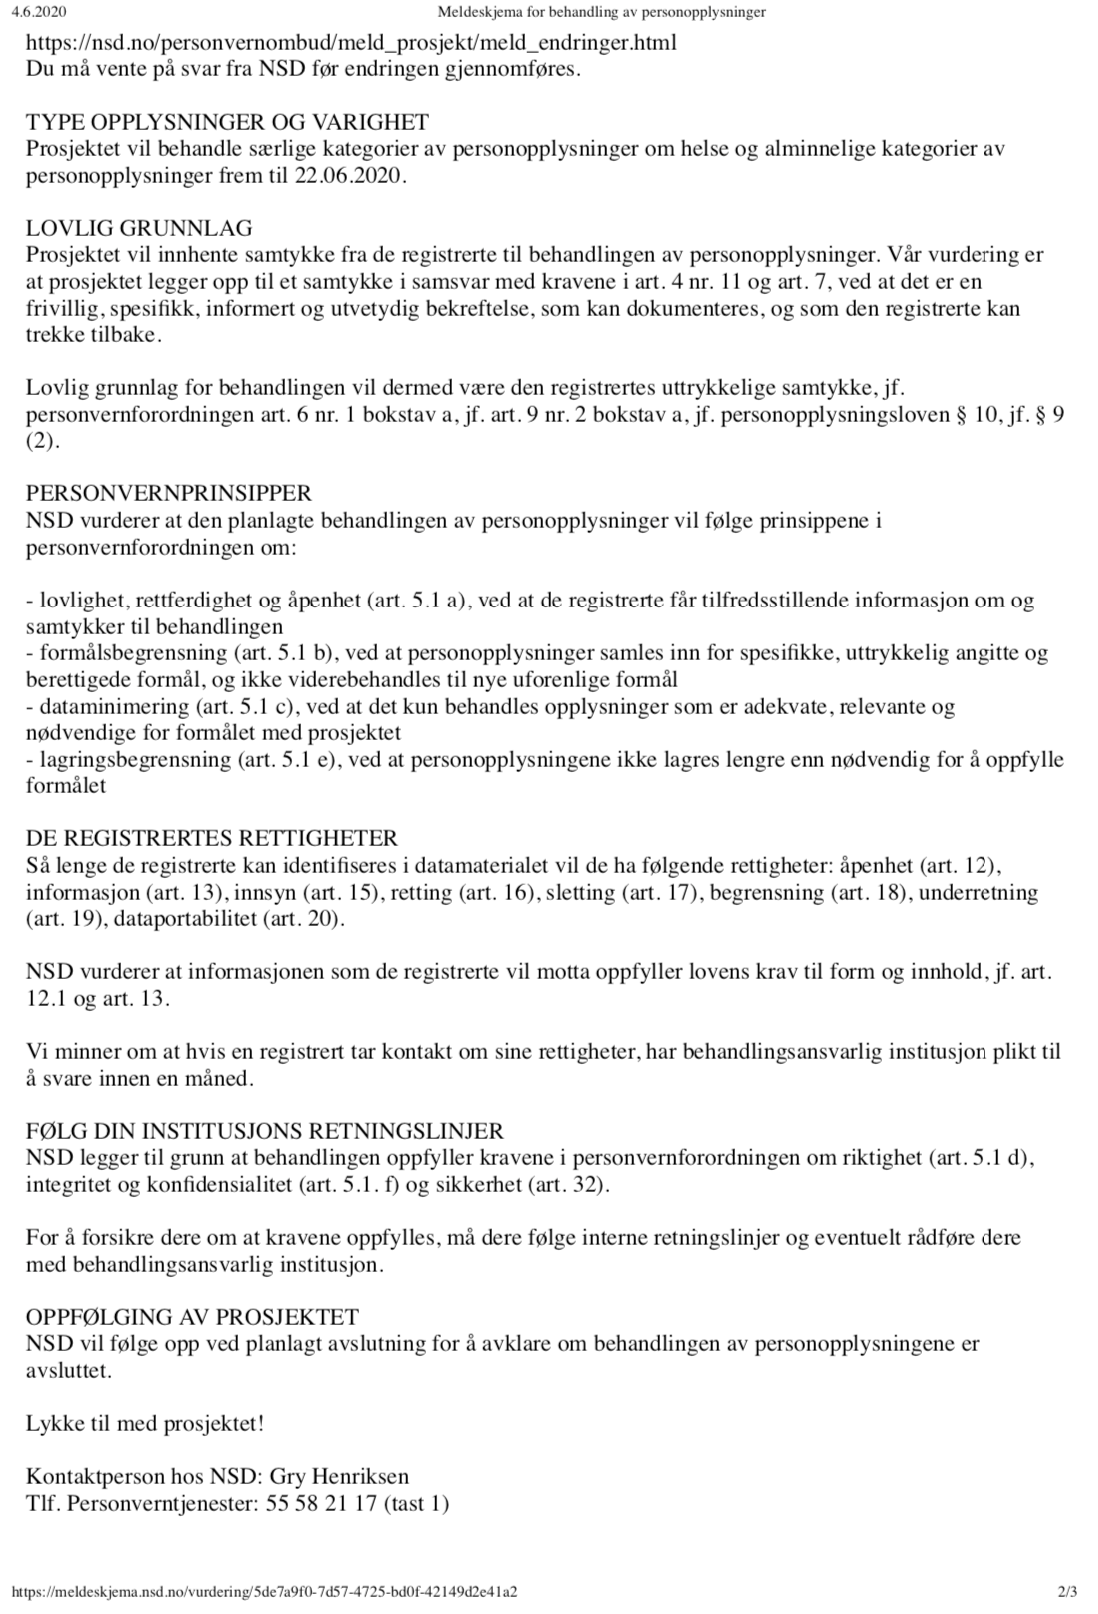
\includegraphics[width=1\textwidth]{images/MS2.png}
\end{figure}

\begin{figure}
    \centering
    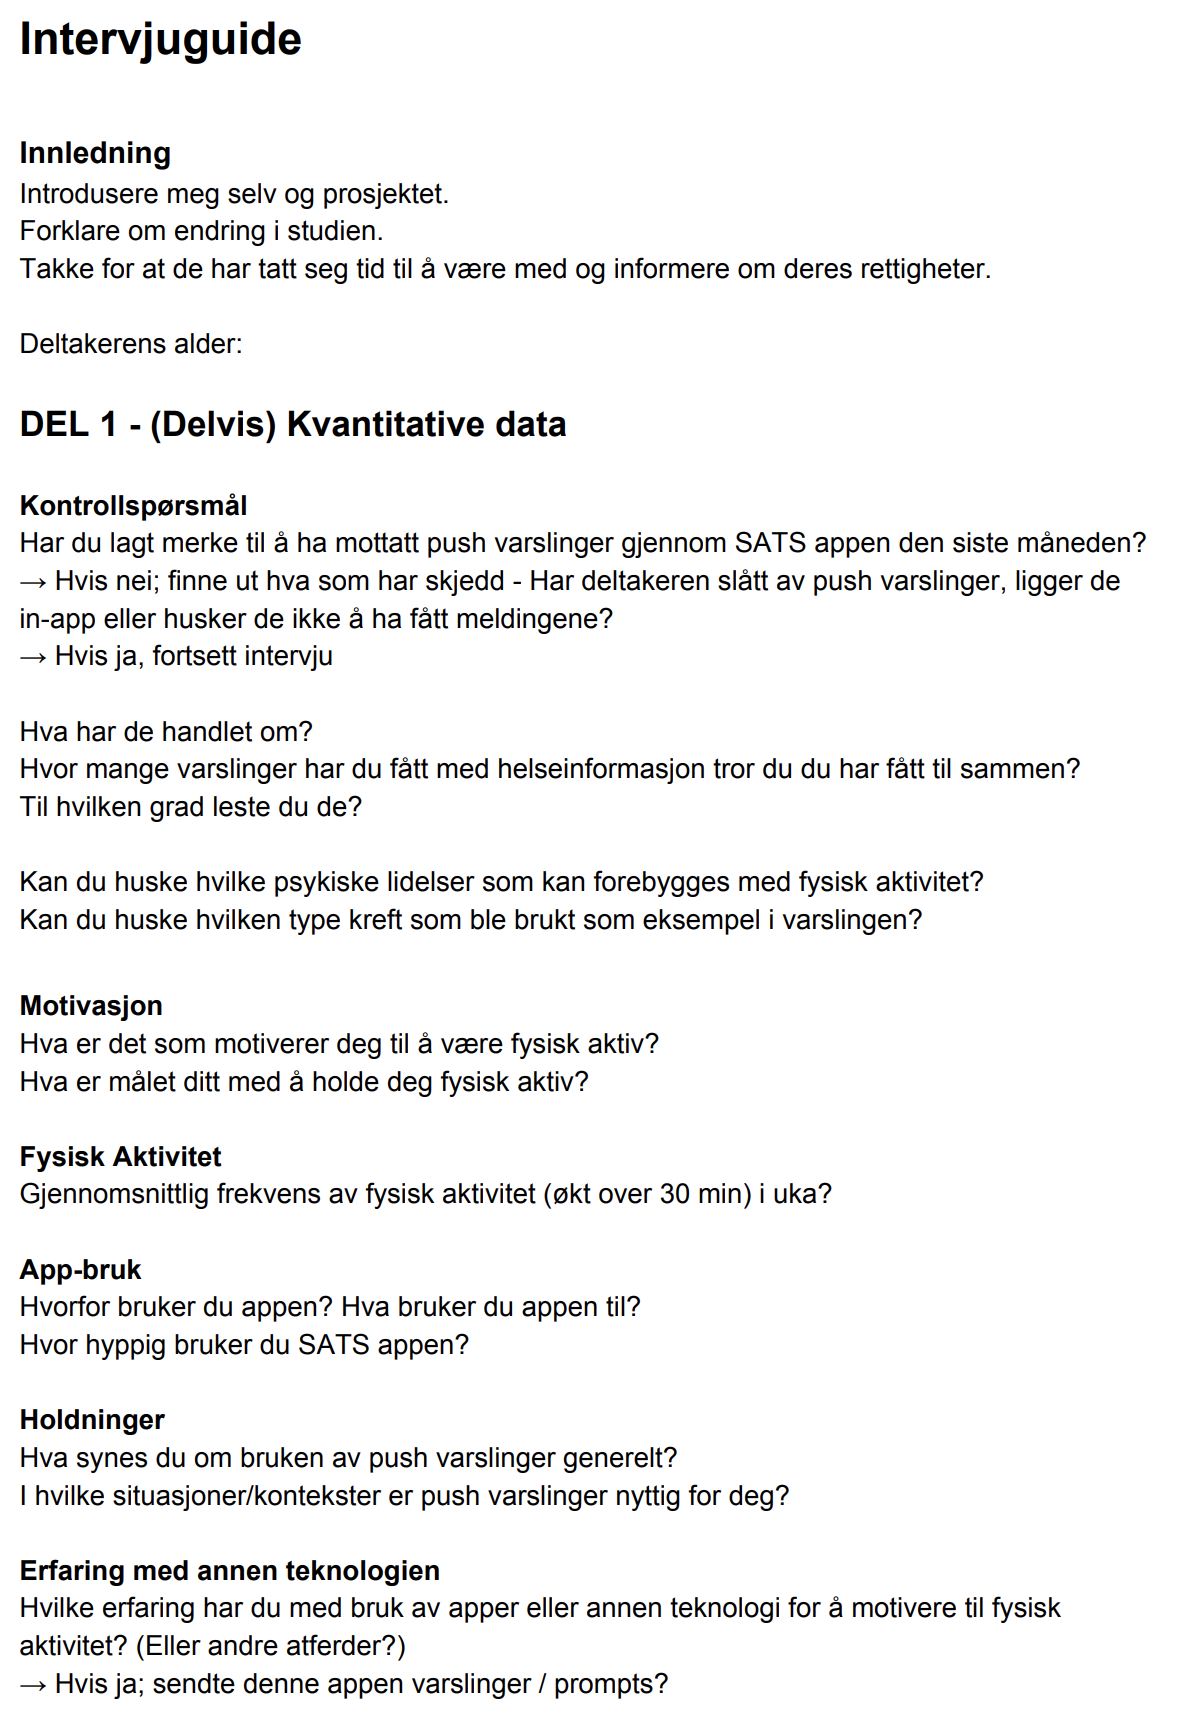
\includegraphics[width=1\textwidth]{images/IG1.png}
\end{figure}

\begin{figure}
    \centering
    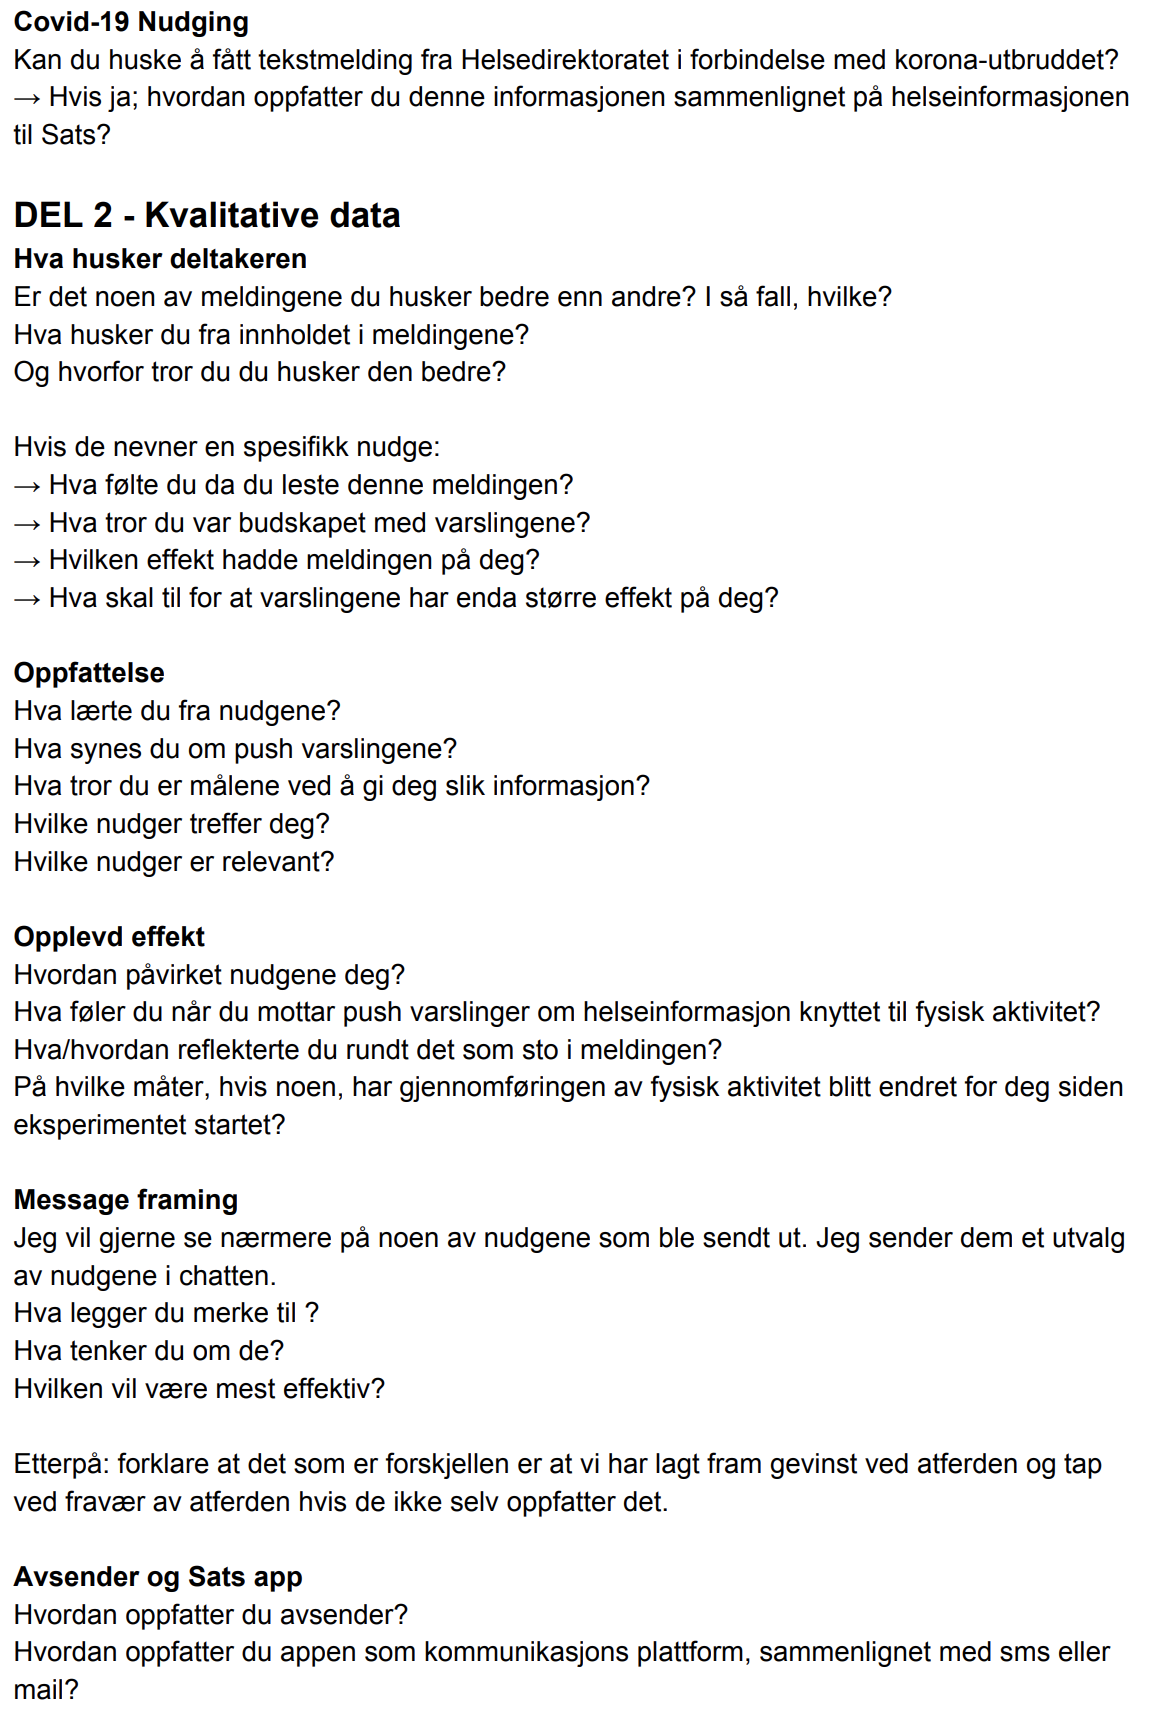
\includegraphics[width=1\textwidth]{images/IG2.png}
\end{figure}



\end{document}
